\documentclass[aps,preprint,preprintnumbers,nofootinbib,showpacs,prd]{revtex4-1}
\usepackage{graphicx,color}
\usepackage{caption}
\usepackage{subcaption}
\usepackage{amsmath,amssymb}
\usepackage{multirow}
\usepackage{amsthm}%        But you can't use \usewithpatch for several packages as in this line. The search 

\usepackage{cancel}

%%% for SLE
\usepackage{dcolumn}   % needed for some tables
\usepackage{bm}        % for math
\usepackage{amssymb}   % for math
\usepackage{multirow}
%%% for SLE -End

\usepackage{ulem}
\usepackage{cancel}

\usepackage{hyperref}
\usepackage{mathrsfs}
\usepackage[top=1in, bottom=1.25in, left=1.1in, right=1.1in]{geometry}

\usepackage{mathtools} % for \DeclarePairedDelimiter{\ceil}{\lceil}{\rceil}

%\usepackage{xeCJK}
%\setCJKmainfont{SimSun}

\newcommand{\msout}[1]{\text{\sout{\ensuremath{#1}}}}


%%%%%% My stuffs - Stef
\newcommand{\lsim}{\mathrel{\mathop{\kern 0pt \rlap
  {\raise.2ex\hbox{$<$}}}
  \lower.9ex\hbox{\kern-.190em $\sim$}}}
\newcommand{\gsim}{\mathrel{\mathop{\kern 0pt \rlap
  {\raise.2ex\hbox{$>$}}}
  \lower.9ex\hbox{\kern-.190em $\sim$}}}

%
% Key
%
\newcommand{\key}[1]{\medskip{\sffamily\bfseries\color{blue}#1}\par\medskip}
%\newcommand{\key}[1]{}
\newcommand{\q}[1] {\medskip{\sffamily\bfseries\color{red}#1}\par\medskip}
\newcommand{\comment}[2]{{\color{red}{{\bf #1:}  #2}}}


\newcommand{\ie}{{\it i.e.} }
\newcommand{\eg}{{\it e.g.} }

%
% Energy scales
%
\newcommand{\ev}{{\,{\rm eV}}}
\newcommand{\kev}{{\,{\rm keV}}}
\newcommand{\mev}{{\,{\rm MeV}}}
\newcommand{\gev}{{\,{\rm GeV}}}
\newcommand{\tev}{{\,{\rm TeV}}}
\newcommand{\fb}{{\,{\rm fb}}}
\newcommand{\ifb}{{\,{\rm fb}^{-1}}}

%
% SUSY notations
%
\newcommand{\neu}{\tilde{\chi}^0}
\newcommand{\neuo}{{\tilde{\chi}^0_1}}
\newcommand{\neut}{{\tilde{\chi}^0_2}}
\newcommand{\cha}{{\tilde{\chi}^\pm}}
\newcommand{\chao}{{\tilde{\chi}^\pm_1}}
\newcommand{\chaop}{{\tilde{\chi}^+_1}}
\newcommand{\chaom}{{\tilde{\chi}^-_1}}
\newcommand{\Wpm}{W^\pm}
\newcommand{\chat}{{\tilde{\chi}^\pm_2}}
\newcommand{\smu}{{\tilde{\mu}}}
\newcommand{\smur}{\tilde{\mu}_R}
\newcommand{\smul}{\tilde{\mu}_L}
\newcommand{\sel}{{\tilde{e}}}
\newcommand{\selr}{\tilde{e}_R}
\newcommand{\sell}{\tilde{e}_L}
\newcommand{\smurl}{\tilde{\mu}_{R,L}}

\newcommand{\casea}{\texttt{IA}}
\newcommand{\caseb}{\texttt{IB}}
\newcommand{\casec}{\texttt{II}}

\newcommand{\caseasix}{\texttt{IA-6}}

%
% Greek
%
\newcommand{\es}{{\epsilon}}
\newcommand{\sg}{{\sigma}}
\newcommand{\dt}{{\delta}}
\newcommand{\kp}{{\kappa}}
\newcommand{\lm}{{\lambda}}
\newcommand{\Lm}{{\Lambda}}
\newcommand{\gm}{{\gamma}}
\newcommand{\mn}{{\mu\nu}}
\newcommand{\Gm}{{\Gamma}}
\newcommand{\tho}{{\theta_1}}
\newcommand{\tht}{{\theta_2}}
\newcommand{\lmo}{{\lambda_1}}
\newcommand{\lmt}{{\lambda_2}}
%
% LaTeX equations
%
\newcommand{\beq}{\begin{equation}}
\newcommand{\eeq}{\end{equation}}
\newcommand{\bea}{\begin{eqnarray}}
\newcommand{\eea}{\end{eqnarray}}
\newcommand{\ba}{\begin{array}}
\newcommand{\ea}{\end{array}}
\newcommand{\bit}{\begin{itemize}}
\newcommand{\eit}{\end{itemize}}

\newcommand{\nbea}{\begin{eqnarray*}}
\newcommand{\neea}{\end{eqnarray*}}
\newcommand{\nbeq}{\begin{equation*}}
\newcommand{\neeq}{\end{equation*}}

\newcommand{\no}{{\nonumber}}
\newcommand{\td}[1]{{\widetilde{#1}}}
\newcommand{\sqt}{{\sqrt{2}}}
%
\newcommand{\me}{{\rlap/\!E}}
\newcommand{\met}{{\rlap/\!E_T}}
\newcommand{\rdmu}{{\partial^\mu}}
\newcommand{\gmm}{{\gamma^\mu}}
\newcommand{\gmb}{{\gamma^\beta}}
\newcommand{\gma}{{\gamma^\alpha}}
\newcommand{\gmn}{{\gamma^\nu}}
\newcommand{\gmf}{{\gamma^5}}
%
% Roman expressions
%
\newcommand{\br}{{\rm Br}}
\newcommand{\sign}{{\rm sign}}
\newcommand{\Lg}{{\mathcal{L}}}
\newcommand{\M}{{\mathcal{M}}}
\newcommand{\tr}{{\rm Tr}}

\newcommand{\msq}{{\overline{|\mathcal{M}|^2}}}

%
% kinematic variables
%
%\newcommand{\mc}{m^{\rm cusp}}
%\newcommand{\mmax}{m^{\rm max}}
%\newcommand{\mmin}{m^{\rm min}}
%\newcommand{\mll}{m_{\ell\ell}}
%\newcommand{\mllc}{m^{\rm cusp}_{\ell\ell}}
%\newcommand{\mllmax}{m^{\rm max}_{\ell\ell}}
%\newcommand{\mllmin}{m^{\rm min}_{\ell\ell}}
%\newcommand{\elmax} {E_\ell^{\rm max}}
%\newcommand{\elmin} {E_\ell^{\rm min}}
\newcommand{\mxx}{m_{\chi\chi}}
\newcommand{\mrec}{m_{\rm rec}}
\newcommand{\mrecmin}{m_{\rm rec}^{\rm min}}
\newcommand{\mrecc}{m_{\rm rec}^{\rm cusp}}
\newcommand{\mrecmax}{m_{\rm rec}^{\rm max}}
%\newcommand{\mpt}{\rlap/p_T}

%%%song
\newcommand{\cosmax}{|\cos\Theta|_{\rm max} }
\newcommand{\maa}{m_{aa}}
\newcommand{\maac}{m^{\rm cusp}_{aa}}
\newcommand{\maamax}{m^{\rm max}_{aa}}
\newcommand{\maamin}{m^{\rm min}_{aa}}
\newcommand{\eamax} {E_a^{\rm max}}
\newcommand{\eamin} {E_a^{\rm min}}
\newcommand{\eaamax} {E_{aa}^{\rm max}}
\newcommand{\eaacusp} {E_{aa}^{\rm cusp}}
\newcommand{\eaamin} {E_{aa}^{\rm min}}
\newcommand{\exxmax} {E_{\neuo \neuo}^{\rm max}}
\newcommand{\exxcusp} {E_{\neuo \neuo}^{\rm cusp}}
\newcommand{\exxmin} {E_{\neuo \neuo}^{\rm min}}
%\newcommand{\mxx}{m_{XX}}
%\newcommand{\mrec}{m_{\rm rec}}
\newcommand{\erec}{E_{\rm rec}}
%\newcommand{\mrecmin}{m_{\rm rec}^{\rm min}}
%\newcommand{\mrecc}{m_{\rm rec}^{\rm cusp}}
%\newcommand{\mrecmax}{m_{\rm rec}^{\rm max}}
%%%song

\newcommand{\mc}{m^{\rm cusp}}
\newcommand{\mmax}{m^{\rm max}}
\newcommand{\mmin}{m^{\rm min}}
\newcommand{\mll}{m_{\mu\mu}}
\newcommand{\mllc}{m^{\rm cusp}_{\mu\mu}}
\newcommand{\mllmax}{m^{\rm max}_{\mu\mu}}
\newcommand{\mllmin}{m^{\rm min}_{\mu\mu}}
\newcommand{\mllcusp}{m^{\rm cusp}_{\mu\mu}}
\newcommand{\elmax} {E_\mu^{\rm max}}
\newcommand{\elmin} {E_\mu^{\rm min}}
\newcommand{\elmaxw} {E_W^{\rm max}}
\newcommand{\elminw} {E_W^{\rm min}}
\newcommand{\R} {{\cal R}}

\newcommand{\ewmax} {E_W^{\rm max}}
\newcommand{\ewmin} {E_W^{\rm min}}
\newcommand{\mwrec}{m_{WW}}
\newcommand{\mwrecmin}{m_{WW}^{\rm min}}
\newcommand{\mwrecc}{m_{WW}^{\rm cusp}}
\newcommand{\mwrecmax}{m_{WW}^{\rm max}}

\newcommand{\mpt}{{\rlap/p}_T}
% \def overrides \Im
\def\Im{{\rm Im}}
\newcommand{\re}{{\rm Re}}

%%%%%% END My stuffs - Stef

\newcommand{\dunno}{$ {}^{\mbox {--}}\backslash(^{\rm o}{}\underline{\hspace{0.2cm}}{\rm o})/^{\mbox {--}}$}

\DeclarePairedDelimiter{\ceil}{\lceil}{\rceil}
\DeclarePairedDelimiter{\floor}{\lfloor}{\rfloor}

%\DeclareMathOperator{\re}{Re}


\begin{document}

\title{Harold Edwards Riemann's zeta function}
\bigskip
\author{Stefanus Koesno$^1$\\
$^1$ Somewhere in California\\ San Jose, CA 95134 USA\\
}
%
\date{\today}
%
\begin{abstract}

\end{abstract}
%
\maketitle

\renewcommand{\theequation}{A.\arabic{equation}}  % redefine the command that creates the equation no.
\setcounter{equation}{0}  % reset counter 

{\bf Page 4}. Footnote, 
%
\nbea
\int_2^L \frac{1}{\log t}dt \sim \frac{L}{\log L}
\neea
%
We might be able to do this using repeated IBPs, with $u = 1/\log t$ and $dv = dt$
%
\nbea
\int_2^L \frac{1}{\log t}dt & = & \left. \frac{t}{\log t}\right|_{2}^{L} + \int_2^L \frac{1}{\log^2 t}dt \\
& = & \frac{L}{\log L} + C_1 + \int_2^L \frac{1}{\log^2 t}dt
\neea
%
we can either repeat the process or do the following
%
\nbea
\int_2^L \frac{1}{\log^2 t}dt & < & \int_2^{L^{1/2}} \frac{1}{\log^2 2}dt + \int_{L^{1/2}}^L \frac{1}{\log^2 L^{1/2}}dt \\
& < & \frac{L^{1/2} - 2}{\log^2 2}  + \frac{L-L^{1/2}}{\log^2 L^{1/2}} \\
& < & \frac{L^{1/2}}{\log^2 2}  + \frac{L}{\log^2 L^{1/2}}
\neea
%
such that
%
\nbea
\int_2^L \frac{1}{\log t}dt & < & \frac{L}{\log L} + C_1 + C_2 L^{1/2} + \frac{L}{\frac{1}{4}\log^2 L}
\neea
%
if we divide both sides by $L/\log L$ and take the limit $L\to\infty$
%
\nbea
\lim_{L\to\infty} \frac{\int_2^L \frac{1}{\log t}dt}{L/\log L} & < & 1 + 0 + \frac{\log L}{L^{1/2}} + \frac{1}{\frac{1}{4}\log L} \\
& < & 1
\neea
%
recall that $\log x$ is smaller than any $x^{1/k}$. But, on the other hand,
%
\nbea
\int_2^L \frac{1}{\log t}dt & > & \int_2^L \frac{1}{\log L}dt \\
& > & \frac{L-2}{\log L} \\
\lim_{L\to\infty} \frac{\int_2^L \frac{1}{\log t}dt}{L/\log L} & > & 1 
\neea
%
thus
%
\nbea
\int_2^L \frac{1}{\log t}dt & \sim & \frac{L}{\log L}
\neea
%
A small note, this asymptotic equality is not like a normal equality, it is more like a Big Oh, say
%
\nbea
f(L) \sim L + L^{1/2}
\neea
%
we can also say
%
\nbea
f(L) \sim L
\neea
%
because $L^{1/2}/L$ approaches zero when $L\to\infty$, so if we divide both sides by $L$ and then take $L\to\infty$ we get the previous asymptotic expression.

{\bf Page 8}. The Gamma function shown here $\Pi(s)$ is valid for all $s > -1$, how is this so as
%
\nbea
\int_0^\infty e^{-x} x^{s} dx
\neea
%
blows up for $s < 0$ when $x\to0$. The justification is as follows
%
\nbea
e^{-x} x^{s} \le x^s
\neea
%
for all $x > 0$ no matter what $s$ is so the integral is also capped by ($s > -1$)
%
\nbea
\int_0^1 e^{-x}x^s dx \le \int_0^1 x^s dx & = & \left.\frac{1}{s+1} x^{s+1} \right|_0^1 \\
& = & \frac{1}{s+1}
\neea
%
Another way of looking at it is
%
\nbea
\int_0^\infty e^{-x}x^n dx & = & e^{-x}\frac{1}{n+1}x^{n+1} + \int_0^\infty e^{-x}\frac{1}{n+1}x^{n+1} dx
\neea
%
so as long as $n>-1$ we are fine.


{\bf Page 8}. On the definition of factorial, Euler introduced the integral notation
%
\nbea
n! & = & \int_0^\infty e^{-x} x^n dx
\neea
%
the $e^{-x}$ is there to make sure everything is well behaved at $\infty$, the $x^n$ is there to be IBP'd (differentiated) multiple times so that we get the factor $n!$, they also make sure that the boundary terms are zero.

But Euler had other ideas too, instead of assigning $x^n \to u$ and differentiating it every IBP, we can instead integrate it, \ie assign $x^n dx \to dv$ like so (boundary terms are always zero and also changing $n\to s$)
%
\nbea
\int_0^\infty e^{-x} x^s dx & = & \frac{1}{s+1} \int_0^\infty e^{-x} x^{(s+1)} dx
\neea
%
repeating it $N$ times we get
%
\nbea
\int_0^\infty e^{-x} x^s dx & = & \frac{1}{(s+1)(s+2) \dots (s+N)} \int_0^\infty e^{-x} x^{(s+N)} dx
\neea
%
and this way we can immediately see the poles at $s = -1, -2, \dots$. We now expand the integral in the RHS above in an interesting way, please do no do IBP by differentiating $x^{(s+n)}$ that will undo everything we've just done. There is, however, a curious way to expand it which only works when $N\to\infty$, we write
%
\nbea
(s + N)! & = & N! \cdot (1 + N)(2 + N) \cdots (s+N)
\neea
%
since $s$ is just a (fixed) parameter, it's finite, and so as we take $N\to\infty$
%
\nbea
\lim_{N\to\infty} (1 + N)(2 + N) \cdots (s+N) & \sim & (1 + N)(1 + N) \cdots (1+N) = (1+N)^s
\neea
%
and thus
%
\nbea
\lim_{N\to\infty}\int_0^\infty e^{-x} x^{(s+N)} dx & = & N! (1+N)^s
\neea
%
So, Euler's definition of a factorial was
%
\nbea
s! & = & \lim_{N\to\infty} \frac{1\cdot2\cdots N}{(s+1)(s+2) \dots (s+N)} (1+N)^s
\neea
%
although whether he got it from the integral above or not I don't know.

{\bf Page 9}.
%
\nbea
\int_0^\infty e^{-nx} x^{s-1} dx & = & \frac{(s-1)!}{n^s} \\
\to \sum_{n=1}^\infty \int_0^\infty e^{-nx} x^{s-1} dx & = & \sum_{n=1}^\infty \frac{(s-1)!}{n^s} \\
& = & (s-1)!\sum_{n=1}^\infty \frac{1}{n^s}
\neea
%
so as long as $s > 1$ the sum of the integral converges, now we want to see the other way, summing inside the integral. A few points
%
\bit
\item Swapping sum and integral is always OK, as long as the sum is finite, for infinite sums what we are interchanging are actually limit and integral because $\sum^\infty = \lim_{N\to\infty}\sum^N$
%
\item Geometric series formula is only valid if the sum converges, why? because we start with
%
\nbea
A & = & 1 + r + r^2 + \dots \\
rA & = & r + r^2 + r^3 + \dots
\neea
%
we then substract $A - rA = 1\to A = 1/(1-r)$ and so on, the problem is if $A$ is divergent we are then doing $\infty - \infty$ which might not be equal to one, so if we try to do $A = 1 + 2 + 2^2 + \dots$ using the formula we get $-1$ which is not just wrong but also not divergent (although if you read Stopple's book you can actually do this and it's called Abel sum).

So the point is that we can't just apply the formula and then take the limit $r\to a$, we can only do this if $a = 1$.
\eit
%

Swapping integral and sum
%
\nbea
\int_0^\infty \sum_{n=1}^\infty e^{-nx} x^{s-1} dx & = & \int_0^\infty \left(\sum_{n=1}^\infty e^{-nx}\right) x^{s-1} dx \\
& = & \int_0^\infty \left (\frac{1}{1-e^{-x}} - 1 \right ) x^{s-1} dx \\
& = & \int_0^\infty \left (\frac{e^{-x}}{1-e^{-x}}\right ) x^{s-1} dx \\
& = & \int_0^\infty \frac{x^{s-1}}{e^{x} - 1} dx
\neea
%
the only problem we have here is when $e^{-x} \ge 1$ and this only happens when $x = 0$, so we only have one point of contention, literally, by the way, this is similar to the situation for
%
\nbea
\int_0^1 \frac{1}{\sqrt{x}} dx & = & 2
\neea
%
even though it blows up at $x = 0$, we do this by
%
\nbea
\int_0^1 \frac{1}{\sqrt{x}} dx & = & \lim_{a\to0}\int_a^1 \frac{1}{\sqrt{x}} dx
\neea
%
in our case the integral is also OK because $e^x - 1 \ge x$ for $x \ge 0$ and so
%
\nbea
\int_0^1 \frac{x^{s-1}}{e^{x} - 1} dx & \le & \int_0^1 x^{s-2} dx \\
& \le & \left. \frac{1}{s-1} x^{s-1} \right |_0^1 \\
& \le & \frac{1}{s-1}
\neea
%
since $s > 1$. Note that we can't just take the limit ($s > 1$)
%
\nbea
\lim_{x\to0} \frac{x^{s-1}}{e^x-1} & = & \lim_{x\to0} \frac{(s-1)x^{s-2}}{e^x} \\
& = & \infty, ~~~~~~~~~~{\rm  since~} s > 1.
\neea
%
so at zero the integrand still blows up but the integral is OK.

{\bf Page 10}. Why the minus sign? the integrand is $\frac{(-x)^s}{e^x - 1}$, there's a minus sign in front of $x$. This is due to the choice of contour. Note that we are going from $+\infty$ to left all the way to 0 and then to the right all the way to $+\infty$.

If there's no minus sign and this is the cut we choose, then
%
\nbea
x^s & = & e^{s\log x + 0\cdot\pi i} , ~~~~~~~~~~ {\rm going~from~} +\infty {\rm ~to~} 0 \\
x^s & = & e^{s\log x + 2\cdot\pi i} , ~~~~~~~~~~ {\rm going~from~} 0 {\rm ~to~} +\infty
\neea
% 
and when we add the two integrals we get zero
%
\nbea
e^{s\log x + 0\cdot\pi i} - e^{s\log x + 2\cdot\pi i} & = & 0
\neea
%
so if we don't want the minus sign we need to choose the other cut, coming from $-\infty$ to zero and back to $-\infty$ so that the phases will be $\pi i$ and $-\pi i$.

{\bf Page 12}. Order of limit taking around the small semi circle, Bernoulli's number, the integral ($x = \delta e^{i\theta}$)
%
\nbea
\int_0^{2\pi} x^{m-n-1} d\theta & = & \frac{\delta^{m-n-1}}{m-n-1} (e^{(m-n-1) \cdot 2\pi \cdot i} - e^{(m-n-1) \cdot 0 \cdot i})
\neea
%
if $m-n-1 < 0$ then the delta term will blow up, but the $e$ difference is zero no matter what, so this means we need to calculate the $e$ difference first before taking the limit.

{\bf Page 13}. Compact here means closed and bounded.

The whole integral is zero thanks to a corollary of Goursat theorem which says that
%
\nbea
\oint_C f(z) dz & = & \sum_{k=1}^n \oint_{C_k} f(z) dz
\neea
%
where the contours $C_k$'s are all inside of $C$.

{\bf Page 13}. For the integral
%
\nbea
\int_{|y|=\epsilon} (-2\pi i n - y)^{s-1} \frac{y}{e^y - 1} \cdot \frac{dy}{y}
\neea
%
we rewrite as
%
\nbea
\int_{|y|=\epsilon} \frac{f(y)}{y - 0} ~ dy, ~~~~~~~~~~ f(y) = (-2\pi i n - y)^{s-1} \frac{y}{e^y - 1}
\neea
%
we need to remember that $f(y)$ has no pole when $y\to 0$, so the value of the integral is just $2\pi i f(0) = 2\pi i(-2\pi i n)^{s-1}$. Note that
%
\nbea
\lim_{y\to0} \frac{y}{e^y - 1} & = & \lim_{y\to0} \frac{1}{e^y} = 1
\neea
%
after L'Hospital.

{\bf Multiple Pages}. A note on analytic continuation. For gamma function, integral is valid only for $s > 1$ but once we get the final form it applies for all $s$. It is even in the derivation of the analytic continuation
%
\nbea
\int_0^\infty e^{-x} x^{s} dx & = & \int_0^1 e^{-x} x^{s} dx + \int_1^\infty e^{-x} x^{s} dx
\neea
%
for the first integral we expand $e$
%
\nbea
\int_0^1 e^{-x} x^{s} dx & = & \int_0^1 \sum_{n=0}^\infty \frac{(-x)^n}{n!} x^{s} dx \\
& = & \sum_{n=0}^\infty (-1)^{n} \int_0^1  \frac{x^{n+s}}{n!} dx
\neea
%
now this integral is not valid for $s \le -1$, however, a this stage we still assume $s > -1$, once we have the full result
%
\nbea
\int_0^\infty e^{-x} x^{s} dx & = & \sum_{n=1}^\infty (-1)^{n-1} \frac{1}{n!(s+n)} + \int_1^\infty e^{-x} x^{s} dx
\neea
%
we say that this result is valid for all $s$, the derivation is not valid for all $s$ but the final result is, that's waht analytic continuation is.

The same goes with the zeta function, in the derivation on Page 10, we take the small semi circle $\delta \to 0$ only for $s > 1$, once we get the final form we say it applies for all $s$ but of course for $s \le 1$ we cannot take $c\to0$ when evaluating the integral, otherwise the integral around that semi circle blows up and we don't have an entire function anymore.

Another remark is that the radius of that small circle must be $0 < \delta < 2\pi$, because at $2\pi i$ we get an infinity from $1/(e^x-1)$.

{\bf Page 15}.
%
\nbea
\frac{1 + 2\psi(x)}{1 + 2\psi(1/x)} = \frac{1}{\sqrt{x}}
\neea
%
for small $x$
%
\nbea
\psi(1/x) & = & \sum e^{-n^2 \pi 1/x} \\
\lim_{x\to 0} \psi(1/x) & = & \sum e^{-n^2 \pi \infty} \\
& = & 0
\neea
%
so for small $x$ we have
%
\nbea
\lim_{x\to 0} \frac{1 + 2\psi(x)}{1 + 2\psi(1/x)} = 1 + 2\psi(x) & = & \frac{1}{\sqrt{x}} \\
\to \psi(x) & = & \frac{1}{2} \left( \frac{1}{\sqrt{x}} - 1\right)
\neea
%

{\bf Page 24}. Fourier transform, I thought I was an expert LOL well, not compared to Riemann
%
\nbea
\int_0^\infty J(x) x^{-s-1} dx & = & \int_0^\infty J(x) x^{-s} \frac{dx}{x}
\neea
%
every time you see $\frac{dx}{x}$ you should immediately scream $\log x$ because $d(\log x) = \frac{dx}{x}$, let $w = \log x$
%
\nbea
\int_0^\infty J(x) x^{-s} \frac{dx}{x} & = & \int_{-\infty}^\infty J(e^w)e^{-ws} dw \\
& = & \int_{-\infty}^\infty J(e^w)e^{-w(\sigma + it)} dw \\
& = & \int_{-\infty}^\infty \left\lbrack J(e^w)e^{-w\sigma} \right\rbrack e^{-itw} dw
\neea
%

{\bf Page 21}. Something I'm not quite sure, ``to prove the absolute convergence of $\prod(1 + a_i)$ it suffices to prove the absolute convergence of the sum $\sum {a_i}$''. To see this, take the log of the product
%
\nbea
\log \prod(1 + a_i) & = & \sum \log(1 + a_i)
\neea
%
But we know that $\log(1 + x) < x$, so if $\sum a_i$ converges then by comparison test the log of the product as well, but if it converges then it converges to a constant and the infinite product is just the exponentiation of a finite constant and thus converges as well.

{\bf Page 25}. Another useful application of IBP, if the integral doesn't converge (in this case due to oscillations), do IBP :)

{\bf Page 26}. about the ambiguity of $\log(1 - s/\rho)$, especially for $\rho$ which are not large, this is because the convention we use is given in Page 27, \ie $\log(z)$ is defined for all $z$ other than real $z \le 0$ and that for real $z$, $\log(z)$ is real.

So if $\rho$ is smaller than $s$ we can have a situation where $(1 - s/\rho)$ is real and negative, but $\log(s-\rho)$ cannot be real and negative when we set $a > 1$ since we know that the zeros are all in the critical strip (see Section 1.9)  and for $\log(-\rho)$, since $\rho$ is never real we are OK since the argument to the log function is never real and negative.

{\bf Page 27}. On the Fourier inversion of $\frac{1}{s-\beta}$, note that the limit of the integration has to go from $-\infty$ to $\infty$, here the function is defined only from $1$ to $\infty$, what this means is that from $-\infty$ to 1 the value of the function is zero.

{\bf Page 28}. Changing variable of integration from the 0 to 1 plus upper semicircle plus 1 to $x$ into $u = \log t$, we see something quite strange. If we change $[0,1]$ using $u = \log t$ we should get $[-\infty,0]$ but instead we get $[-\infty + i\delta, 0 + i\delta]$, in the book the integration is split into $[i\delta-\infty,i\delta+\log x]$.

This is actually more in line to shifting the whole original contour to be slightly above the positive $x$ axis, rather than doing an upper semicircle. If we push it up the argument of the log has to be positive thus the addition of $i\delta$.

{\bf Page 29}. Here we show that $H(\beta)\to0$ as $\tau\to\infty$, but since $H(\beta)$ is extremely similar to $F(\beta)$, the difference is only in the 
%
\nbea
\log\lbrack 1 - (s/\beta)\rbrack \longleftrightarrow \log\lbrack (s/\beta) - 1 \rbrack 
\neea
%
so the key difference here is that for $H(\beta)$, when we take $\tau\to\infty$, we get $\log\lbrack 1 - (s/\beta)\rbrack \to \log(1)$ while for $F(\beta)$ we get $\log(-1)$. And here we see some application of Lebesgue integral that allows us to interchange limit and integration.

Looking back, this might be the exact reason why we introduce $H(\beta)$ in the first place, we know we need to take $\tau\to\infty$ (recall that $\beta = \sigma + i\tau$), but doing this in $F(\beta)$ causes something like $\log(-1)$, if we reverse the sign inside the log, we might be able to get something, but first we need to see if this log reversed function is the same as our original function, the good news is that in this case they are only separated by a constant $i\pi$.

{\bf Page 30}. Pairing $\rho$ and $1-\rho$, in case you forget, this was discussed back on Page 21.

{\bf Page 31}. $-\zeta(0) = \frac{1}{2}$, here we are using Abel's sum or from the Bernoulli number formula thingy
%
\nbea
\zeta(2n) & = & (-1)^{n+1} \frac{(2\pi)^{2n}}{2} \frac{B_{2n}}{2n!}
\neea
%
and setting $n = 0$, a more interesting way is using Abel's sum but not on $\zeta(0)$ directly because
%
\nbea
\zeta(0) & = & 1 + 1 + 1 + \dots \\
& = & \frac{1}{1-1} \\
& = & \infty
\neea
%
instead we do Abel's summation on 
%
\nbea
\Phi(s) & = & (1 - 2^{1-s})\zeta(s) = 1 - \frac{1}{2^s} + \frac{1}{3^s} - \frac{1}{4^s} + \frac{1}{5^s} \dots = \sum_{n=1}\frac{(-1)^{n-1}}{n^s}
\neea
%
the zero $(1 - 2^{1-s})$ at $s = 1$ cancels the pole of $\zeta(s)$ at $s=1$. Now, for $\Phi(s=0)$ we get
%
\nbea
\Phi(0) & = & 1 - 1 + 1 - 1 + 1 \dots \\
& = & \frac{1}{1 + 1} \\
& = & \frac{1}{2}
\neea
%
instead of $\frac{1}{1-1}$ (again, the pole at $s = 1$ was canceled), thus
%
\nbea
\zeta(0) & = & (1 - 2^{1})^{-1} \Phi(0) \\
& = & (-1) \frac{1}{2}
\neea
%

{\bf Page 42}. The curious thing about the application of Jensen's theorem here is that instead of $\xi(0)$ we get $\xi(1/2)$, the thing to note is that the radius used in Jensen's Theorem is $|z| \le R$, here it is $|s-\frac{1}{2}| \le R$, so the prerequisite is not met :)

We just need to do a simple change of variable $w = s - \frac{1}{2}$ and thus $|w| \le R$
%
\nbea
\xi(s) & = & \xi(w + \frac{1}{2}) \\
\to f(w) & = & \xi(w + \frac{1}{2})
\neea
%
and we do Jensen's Theorem on $f(w)$ instead, in this case
%
\nbea
f(w = 0) & = & \xi\left(\frac{1}{2}\right)
\neea
%
and the zeros of $f(w)$ are now located at $\rho-\frac{1}{2}$ where $\xi(\rho) = 0$, all done :)

{\bf Page 42}. This statement, ``Since all but a finite number of roots $\rho$ satisfy the inequality''
%
\nbea
\frac{1}{|\rho(1-\rho)|} = \frac{1}{|(\rho-\frac{1}{2})^2 - \frac{1}{4}|} < \frac{1}{|\rho-\frac{1}{2}|^2}
\neea
%
let $\rho - \frac{1}{2} = a + ib$ then
%
\nbea
|(\rho-\frac{1}{2})^2 - \frac{1}{4}|^2 & = & (a^2 + b^2 - \frac{1}{4}) + 4a^2b^2 \\
|(\rho-\frac{1}{2})^2|^2 & = & (a^2 + b^2)^2
\neea
%
taking the difference
%
\nbea
|(\rho-\frac{1}{2})^2 - \frac{1}{4}|^2 - |(\rho-\frac{1}{2})^2|^2 & = & \frac{(8a^2 - 1)(8b^2 - 1)}{16}
\neea
%
so for $a^2 > \frac{1}{8}$ and $b^2 > \frac{1}{8}$ we get the inequality in the book, thus only for those roots whose $\Re(\rho-\frac{1}{2})^2 < \frac{1}{8}$ or $\Im(\rho-\frac{1}{2})^2 < \frac{1}{8}$ we don't get the inequality in the book.

{\bf Page 43}. Note that this Theorem and the preceding one all rely on the fact that $R$ is sufficiently large, the inequality
%
\nbea
n(R) \le 3R\log R
\neea
%
doesn't work for all $R$, only for $R$ sufficiently large.

Also this is about seeing how dense the roots of $\xi(s)$ are, note that for example $\sum 1/p$, although is not as dense as $\sum 1/n$, still diverges.

{\bf Page 44}. Dealing with $u_R(s)$, we invoke properties of harmonic functions, first a harmonic function is just a holomorphic function because it is a function that satisfies Cauchy-Riemann conditions, or in other words it satisfies Laplace's equation
%
\nbea
\partial_x^2 f + \partial_y^2 f & = & 0
\neea
%
and because of this very reason a harmonic function cannot have a max or min within a compact domain, because if $x$ is a max/min then it's second derivative in $x$ must be non-zero but due to Laplace's equation above the second derivative in the $y$ has the opposite sign and therefore it is a saddle point.

In this case the domain is not really compact because we exclude the zeros of $\xi$, this is why the book explains that near this point the value is near $-\infty$, so there's no chance to have a max point near these points and the max points should be at the boundary.

{\bf Page 46}. $F(s)$ is an even function of $s - \frac{1}{2}$. We know that $\xi(s)$ is symmetric under $s\to 1-s$, thus
%
\nbea
\frac{\xi(1-s)}{\prod \left \lbrack 1 - \frac{(1-s) - \frac{1}{2}}{\rho - \frac{1}{2}}\right \rbrack} & = & \frac{\xi(s)}{\prod \left \lbrack 1 - \frac{\frac{1}{2}-s}{\rho - \frac{1}{2}}\right \rbrack}
\neea
%
However, if $\rho$ is a zero then $1 - \rho$ is also a zero, thus
%
\nbea
\frac{\xi(s)}{\prod \left \lbrack 1 - \frac{\frac{1}{2}-s}{\rho - \frac{1}{2}}\right \rbrack} & = & \frac{\xi(s)}{\prod \left \lbrack 1 - \frac{\frac{1}{2}-s}{\frac{1}{2} - \rho}\right \rbrack} = \frac{\xi(s)}{\prod \left \lbrack 1 - \frac{-(s - \frac{1}{2})}{-(\rho-\frac{1}{2})}\right \rbrack} = \frac{\xi(s)}{\prod \left \lbrack 1 - \frac{s - \frac{1}{2}}{\rho-\frac{1}{2}}\right \rbrack}
\neea
%
which is all good and all but this is a symmetry under $s\to1-s$, to make it into a symmetry under $s - \frac{1}{2}$ we do the following
%
\nbea
\xi(s) & = & \xi((s - \frac{1}{2}) + \frac{1}{2})
\neea
%
so that under $s - \frac{1}{2} \to \frac{1}{2} - s$ we get
%
\nbea
\xi((s - \frac{1}{2}) + \frac{1}{2}) & \to & \xi((\frac{1}{2} - s) + \frac{1}{2}) \\
& = & \xi(1 - s) \\
& = & \xi(s) \\
& = & \xi((s - \frac{1}{2}) + \frac{1}{2})
\neea
%

{\bf Page 47}. Footnote, first the validity of the product formula for $\sin \pi s$, note that it is easier to show the validity of the product formula for $\frac{\sin \pi s}{\pi s}$, using the Theorem in Section 2.7, we see that $\left (\frac{\sin \pi s}{\pi s}\right )/\left (\prod \left \lbrack 1 - \frac{s^2}{n^2}\right \rbrack \right )$ is an even function and it does grow more slowly than $|s|^2$. Thus
%
\nbea
\frac{\sin \pi s}{\pi s} & = & c \prod \left ( 1 - \frac{s}{n} \right ) \left ( 1 + \frac{s}{n} \right ) \\
& = & c \prod \left ( 1 - \frac{s^2}{n^2} \right )
\neea
%
where we have paired the roots to ensure the infinite product is convergent. Next
%
\nbea
\frac{(\sin \pi s)/(\pi s)}{(\sin \pi 0)/(\pi 0)} & = & \frac{\prod \left ( 1 - \frac{s^2}{n^2} \right )}{1}
\neea
%
But $(\sin \pi 0)/(\pi 0) = 1$ thus
%
\nbea
\frac{\sin \pi s}{\pi s} & = & \prod \left ( 1 - \frac{s^2}{n^2} \right )
\neea
%
The second footnote is not related to this one, it just says that everything in that page has been rigorously proven, including the product formula for sin, the only thing not proven is the relationship between (2) and (3).

{\bf Page 50}. Footnote, logarithmic differentiation of $\zeta(s)$
%
\nbea
\frac{d(\log \zeta(s))}{ds} = \frac{\zeta'(s)}{\zeta(s)} & = & \frac{d}{ds} \left ( \log\prod (1 - p^{-s})^{-1}\right ) \\
& = & -\sum_p \frac{d}{ds} \log(1 - p^{-s}) \\
& = & -\sum_p \frac{\log p}{1 - p^{-s}}
\neea
%
then
%
\nbea
\frac{1}{1 - p^{-s}} & = & 1 + p^{-s} + p^{-2s} + \dots
\neea
%
so
%
\nbea
-\sum \frac{\log p}{1 - p^{-s}} & = & -\sum_p \log p \sum_k p^{-ks}
\neea
%
and we are done :)

{\bf Page 51}. formula (2) of Section 1.14 is
%
\nbea
\frac{1}{2\pi i} \int_{a - i\infty}^{a + i\infty} \frac{1}{s - \beta} y^s ds & = & \left \{
\begin{array}{ll}
y^\beta &~~~~~ y > 1 \\
0 &~~~~~ y < 1
\end{array}
\right.
\neea
%



{\bf Page 52}. Bottom page, about the middle equation, say $\beta = A + iB$, here we don't take the limit $h\to\infty$ yet
%
\nbea
\int_{a - \beta - ih}^{a - \beta + ih} & = & \int_{a - A - iB - ih}^{a - A - iB + ih} \\
& = & \int_{a - A - iB - ih}^{a - A - ih} + \int_{a - A - ih}^{a - A + ih} + \int_{a - A + ih}^{a - A -iB + ih} \\
& = & \int_{a - A - iB - ih}^{a - A - ih} + \int_{\Re{(a - \beta)} - ih}^{\Re{(a - \beta)} + ih} + \int_{a - A + ih}^{a - A -iB + ih} 
\neea
%
so now we have to make sure that these side band integrals are negligible, let $t = a - A + i\tau$
%
\nbea
\int_{a - A + ih}^{a - A -iB + ih}  \frac{x^t}{t} dt & = & i\int_{h}^{(h - B)} \frac{e^{(a-A+i\tau)\log x}}{a -  A + i\tau} d\tau \\
& \le & \int_{h}^{(h - B)} \frac{|e^{(a-A+i\tau)\log x}|}{|a -  A + i\tau|} d\tau \\
& \le & e^{a - A} \int_{h}^{(h - B)} \frac{1}{|i\tau|} d\tau \\
& \le & e^{a - A} \log (1 - \frac{B}{h})
\neea
%
if we take the limit $h\to\infty$ we get $\to\log 1$ which approaches zero :) we can do the same with the lower side band and get the same result. The lesson here is that we don't need exact things, \ie we don't need it to be exactly zero, approaching zero is good enough and this I see over and over in analytic number theory.

{\bf Multiple Pages}. I find it interesting that to prove that the limit of the sum is the sum of the limit we just need to show that the latter converges but we did not need to show that they converge to the same value.

{\bf Page 55}. The integrand in the second integral is an odd function
%
\nbea
i\int_{-h}^{h} \frac{t}{a^2 + t^2} dt
\neea
%
and it's integrated in a symmetric domain so the integral is zero :)

{\bf Page 55}. This is the normal trig trick :)
%
\nbea
\int \frac{1}{1+u^2} du & = & \int \frac{1}{1 + \tan^2 w} \frac{dw}{\sec^2 w}, ~~~~~ \frac{1}{1 + \tan^2 w} = \sec^2 w \\
& = & \int dw \\
& = & w = \arctan u
\neea
%

{\bf Page 56}. Inequality on first line
%
\nbea
(a - c)^2 = a^2 - 2ac + c^2 & > & 0 \\
a^2 + c^2 & > & 2ac \\
2(a^2 + c^2) & > & a^2 + 2ac + c^2 \\
a^2 + c^2 & > & \frac{(a+c)^2}{2} \\
\sqrt{a^2 + c^2} & > & \frac{(a+c)}{\sqrt{2}} \\
\to |a + ic| & > & \frac{(a+c)}{\sqrt{2}}
\neea
%

{\bf Page 58}. And again, just for fun
%
\nbea
\cos \frac{\pi}{4} = \cos 2 \frac{\pi}{8} & = & 2 \cos^2 \frac{\pi}{8} - 1 \\
\frac{1}{\sqrt{2}} & = & 2 \cos^2 \frac{\pi}{8} - 1 \\
\to \cos \frac{\pi}{8} & = & \left(\frac{1 + \frac{1}{\sqrt{2}}}{2}\right)^{1/2}
\neea
%
by the same token
%
\nbea
\cos \frac{\pi}{4} = \cos 2 \frac{\pi}{8} & = & 1 - 2 \sin^2 \frac{\pi}{8} \\
\to \sin \frac{\pi}{8} & = & \left(\frac{1 - \frac{1}{\sqrt{2}}}{2}\right)^{1/2}
\neea
%
and so
%
\nbea
\tan \frac{\pi}{8} & = & \left (\frac{\frac{1 - \frac{1}{\sqrt{2}}}{2}}{\frac{1 + \frac{1}{\sqrt{2}}}{2}} \right )^{1/2} = \left (\frac{1 - \frac{1}{\sqrt{2}}}{1 + \frac{1}{\sqrt{2}}} \right )^{1/2} = \left (\frac{1 - \frac{1}{\sqrt{2}}}{1 + \frac{1}{\sqrt{2}}} \times \frac{1 + \frac{1}{\sqrt{2}}}{1 + \frac{1}{\sqrt{2}}}\right )^{1/2} \\
& = & \left(\frac{1 - \frac{1}{2}}{\left(1 + \frac{1}{\sqrt{2}}\right)^2} \right) ^{1/2} = \frac{1}{1 + \frac{1}{\sqrt{2}}}\cdot \frac{1}{\sqrt{2}} = \frac{1}{1 + \sqrt{2}} < \frac{1}{2}
\neea
%

{\bf Page 65}. Evaluating integrals
%
\nbea
\int_0^K \frac{1}{r-1} dr
\neea
%
there's a pole here at $r = 1$, this is almost the same as integrating $dz/z$, so let's make the change of variable $z = r-1, dz = dr$
%
\nbea
\int_0^K \frac{1}{r-1} dr = \int_{-1}^{K-1} \frac{1}{z} dz & = & \int_{-1}^{0-\delta} \frac{1}{z} dz  + \int_C \frac{1}{z} dz + \int_{0+\delta}^{K-1} \frac{1}{z} dz
\neea
%
where the contour $C$ for the middle integral is an upper semicircle above $z = 0$, 
%
\nbea
\int_C \frac{1}{z} dz & = & \int_{\pi}^{0} \frac{1}{\delta e^{i\theta}} d(\delta e^{i\theta}) \\
& = & i\int_{\pi}^{0} \frac{\delta e^{i\theta}}{\delta e^{i\theta}} d\theta \\
& = & -i\pi
\neea
%
Now for the other integrals we do the following
%
\nbea
\int_{-1}^{0-\delta} \frac{1}{z} dz  + \int_{0+\delta}^{K-1} \frac{1}{z} dz & = & \int_{1}^{0+\delta} \frac{1}{-z} d(-z)  + \int_{0+\delta}^{1} \frac{1}{z} dz + \int_{1}^{K-1} \frac{1}{z} dz \\
& = & -\int_{0+\delta}^{1} \frac{1}{z} dz  + \int_{0+\delta}^{1} \frac{1}{z} dz + \int_{1}^{K-1} \frac{1}{z} dz \\
& = & \int_{1}^{K-1} \frac{1}{z} dz
\neea
%
so we first do $z\to-z$ on the first integral and then swap the integration limits, for the second integral we split the integral, this way we can cancel the blowing up parts and are left with $\log(K-1)$.

We can also shift the pole by the usual trick
%
\nbea
\int_{-1}^{K-1} \frac{1}{z} dz \to \int_{-1}^{K-1} \frac{1}{z + i\epsilon} dz & = & \log (K - 1 + i\epsilon) - \log(-1 + i\epsilon)
\neea
%
taking the limit $\epsilon\to0$ is a bit tricky because the log is a bit ambiguous, is $\log (-1) = i \pi$ or $-i\pi$?

{\bf Page 69}. These equations are quite easily derived using von Mangoldt's method :) For me the starting point is Section 3.7, Eq. (1) - (3) which culminates in the following equation 
%
\nbea
\int_0^x t^{-r} d\psi(t) & = & \frac{x^{1-r}}{1-r} - \sum_\rho \frac{x^{\rho-r}}{\rho-r} + \sum_n \frac{x^{-2n-r}}{2n+r} - \frac{\zeta'(r)}{\zeta(r)}
\neea
%
and for what we need
%
\nbea
\int_0^x \left(\frac{x}{t}\right)^{r} d\psi(t) & = & \frac{x}{1-r} - \sum_\rho \frac{x^{\rho}}{\rho-r} + \sum_n \frac{x^{-2n}}{2n+r} - x^r\frac{\zeta'(r)}{\zeta(r)}
\neea
%


If we set $r=0$ we get
%
\nbea
\int_0^x t^{-0} d\psi(t) = \int_0^x t^{-0} d\psi(t) = \int_0^x d\psi(t) = \psi(x) & = & x - \sum_\rho \frac{x^{\rho}}{\rho} + \sum_n \frac{x^{-2n}}{2n} - \frac{\zeta'(0)}{\zeta(0)}
\neea
%
although this still needs all those arguments about swapping sums, integrals and limits :)

To get de la Vallee Poussin's Eq (3) we need the following IBP 
%
\nbea
\int_0^x \log \frac{x}{t} d\psi(t) & = & \left. \log \frac{x}{t} \psi(t) \right|_0^x + \int_0^x t^{-1} \psi(t) dt \\
& = & \psi(x) \log \frac{x}{x} - \psi(0)\log \frac{x}{0} + \int_0^x t^{-1} \psi(t) dt
\neea
%
Note that $\psi(0) = 0$, there's no limit taken here so
%
\nbea
\psi(0)\log \frac{x}{0} & = & \lim_{r\to0} 0 \cdot \log \frac{x}{r}
\neea
%
and therefore it is zero and from the main equation of Section 3.7 as stated above we do the following (differentiating inside the integral)
%
\nbea
\frac{d}{dr}\left.\left(\int_0^x \left(\frac{x}{t}\right)^{r} d\psi(t)\right)\right|_{r = 0} & = & \int_0^x (\log \frac{x}{t}) d\psi(t)\\
\int_0^{x} t^{-1} \psi(t) dt & = & x - \sum_\rho \frac{x^\rho}{\rho^2} - \sum_n \frac{x^{-2n}}{(2n)^2} - \log x \frac{\zeta'(0)}{\zeta(0)}  - \frac{\zeta''(0)\zeta(0) - \zeta'^2(0)}{\zeta^2(0)} \\
\to \int_0^{x} t^{-1} \psi(t) dt & = & x -\sum_\rho \frac{x^\rho}{\rho} - \sum_n \frac{x^{-2n}}{(2n)^2} - \log x\frac{\zeta'(0)}{\zeta(0)} + {\rm const.}
\neea
%
This way we don't need the explicit formula for $\psi(x)$.

For Hadamard's Eq (2) what we need is the footnote on Page 74. First we reuse the (modified) main formula from Page 69, shown above, \ie the formula for $\int_0^x \left(\frac{x}{t}\right)^{r} d\psi(t)$, once we have this, we do the following
%
\nbea
\int_0^x \left(\frac{x}{t}\right)^{r} d\psi(t) - \int_0^x \left(\frac{x}{t}\right)^{w} d\psi(t) & = & \left(\frac{x}{1-r} - \frac{x}{1-w} \right ) - \sum_\rho \left(\frac{x^{\rho}}{\rho-r} - \frac{x^{\rho}}{\rho-w} \right) + \\
&& \sum_n \left(\frac{x^{-2n}}{2n+r} - \frac{x^{-2n}}{2n+w}\right) - \left(x^r\frac{\zeta'(r)}{\zeta(r)} - x^w\frac{\zeta'(w)}{\zeta(w)} \right ) \\
& = & x \frac{(r-w)}{(r-1)(w-1)} - \sum_\rho \frac{x^{\rho} (r-w)}{(\rho-r)(\rho-w)} \\
&& - \sum_n \frac{x^{-2n}(r-w)}{(2n+r)(2n+w)} - \left(x^r\frac{\zeta'(r)}{\zeta(r)} - x^w\frac{\zeta'(w)}{\zeta(w)} \right )
\neea
%
which is the formula given in the footnote, and heeding the footnote :) to get (2) we set $r = 1, w = 0$ and do IBP on the Left Hand Side
%
\nbea
\int_0^x \frac{x}{t} d\psi(t) - \int_0^x d\psi(t) & = &  \left.\frac{x}{t} \psi(t) \right |_0^x + \int_0^x \frac{x}{t^2} \psi(t) dt - \psi(x) \\
& = & \left ( \bcancel{\psi(x)} - \frac{x\psi(x)}{0}\right ) + x \int_0^x t^{-2} \psi(t) dt - \bcancel{\psi(x)} \\
& = & x \int_0^x t^{-2} \psi(t) dt
\neea
%
again $\frac{\psi(0)}{0}$ is zero because $\psi(0) = 0$. The RHS is straightforward, except for the first term, therefore we have to combine this with the last term because these infinities cancel out
%
\nbea
& = & \left (\lim_{r\to1} x \frac{1}{1-r} - x^r\frac{\zeta'(r)}{\zeta(r)} \right) - \sum_\rho \frac{x^{\rho} (1-0)}{(\rho-1)(\rho-0)} - \sum_n \frac{x^{-2n}(1-0)}{(2n+1)(2n+0)} + x^0\frac{\zeta'(0)}{\zeta(0)} \\
& = & \left (\lim_{r\to1} x \frac{1}{1-r} - x^r\frac{\zeta'(r)}{\zeta(r)} \right) - \sum_\rho \frac{x^{\rho}}{(\rho-1)\rho} - \sum_n \frac{x^{-2n}}{(2n+1)2n} + \frac{\zeta'(0)}{\zeta(0)}
\neea
%
the limit is calculated by Laurent expanding $\frac{\zeta'(r)}{\zeta(r)}$ and isolate the pole term, however, we incur an extra minus sign (and it has to for it to work, see Lemma 4 Page 289 of Apostol)
%
\nbea
\lim_{r\to 1}\frac{x}{1-r} - x^r\frac{\zeta'(r)}{\zeta(r)} = \lim_{r\to 1}\frac{x}{1-r} - \frac{x^r}{1-r}  + x^r \cdot f(r) & = & \lim_{r\to1} \frac{x-x^{r}}{1-r} + x^r \cdot f(r) \\
& = & \lim_{r\to1} \frac{-x^r \log x}{-1} + x^r \cdot {\rm const.} \\
& = & x \log x + x \cdot {\rm const.}
\neea
%
Combining everything
%
\nbea
x \int_0^x t^{-2} \psi(t) dt & = & x \log x - \sum_\rho \frac{x^{\rho}}{(\rho-1)\rho} - \sum_n \frac{x^{-2n}}{(2n+1)2n} + \frac{\zeta'(0)}{\zeta(0)} + x \cdot {\rm const.} \\
\to \int_0^x t^{-2} \psi(t) dt & = & \log x - \sum_\rho \frac{x^{\rho-1}}{(\rho-1)\rho} - \sum_n \frac{x^{-2n-1}}{(2n+1)2n} + \frac{1}{x}\frac{\zeta'(0)}{\zeta(0)} + {\rm const.}
\neea
%


{\bf Page 70}. The sum
%
\nbea
B = \frac{1}{2} \sum\frac{1}{p^2} + \frac{1}{3} \sum\frac{1}{p^3} + \frac{1}{4} \sum\frac{1}{p^4} + \dots
\neea
%
converges, this is how, for $k \ge 2$
%
\nbea
\sum \frac{1}{p^k} & < & \sum_{n=2} \frac{1}{n^k} < 1
\neea
%
the last inequality can be easily shown using the integral test which shows that
%
\nbea
\sum_{n=2} \frac{1}{n^k} < \int_1^\infty x^{-k} dx & = & \frac{1}{k - 1}
\neea
%
%
\nbea
B = \frac{1}{2} \sum\frac{1}{p^2} + \frac{1}{3} \sum\frac{1}{p^3} + \frac{1}{4} \sum\frac{1}{p^4} + \dots & < & \frac{1}{2} \sum\frac{1}{n^2} + \frac{1}{3} \sum\frac{1}{n^3} + \frac{1}{4} \sum\frac{1}{n^4} + \dots \\
& < & \frac{1}{2} \cdot1 + \frac{1}{3} \cdot\frac{1}{2} + \frac{1}{4} \cdot \frac{1}{3} + \dots \\
& = & \sum_{n=2}\frac{1}{n(n-1)}
\neea
%
and using the integral test this one is also convergent :)

Here's a way that doesn't work, initially I wanted to show that we can massage $B$ into $\sum \frac{1}{p^s}$ with $s > 1$, this is because each $\sum \frac{1}{p^k}$ is less than one, so there must be an $s > 1$ such that 
%
\nbea
\frac{1}{n}\sum\frac{1}{p^n} & = & \frac{1}{p^s}
\neea
%
however, this $s$ is getting smaller and smaller as $p$ gets bigger and it approaches 1, so if we use the same $s$ for all $p$ we get $\sum \frac{1}{p}$ and it doesn't work.





{\bf Page 73}. One trick to calculate $\int_0^x t^{k-1} \psi(t) dt$ is, one, the partial fraction formula
%
\nbea
\frac{1}{s(s+k)} = \frac{1/k}{s} - \frac{1/k}{s + k}
\neea
%
and from this we can see that to get other powers of $x$ we do the following
%
\nbea
\frac{1}{2\pi i} \int_{a - i\infty}^{a + i\infty} \frac{x^{s+1}}{n^s s (s+1)} ds \to \frac{1}{2\pi i} \int_{a - i\infty}^{a + i\infty} \frac{x^{s+k}}{n^s s (s+k)} ds
\neea
%
splitting through partial fraction
%
\nbea
\frac{x^k}{k 2\pi i} \int_{a - i\infty}^{a + i\infty} \left(\frac{x}{n}\right)^{s} \frac {ds}{s}-\frac{n^k}{k 2\pi i} \int_{a - i\infty}^{a + i\infty} \left(\frac{x}{n}\right)^{s+k} \frac {ds}{s+k}
\neea
%
which becomes
%
\nbea
 = \left\{
 \begin{array}{ ll }
 \frac{1}{k} \left ( x^k - n^k\right ) ~~~~~ & {\rm if~} n \le x \\
 0 ~~~~~ & {\rm if~} n \ge x
 \end{array}
 \right.
\neea
%
so what we have is 
%
\nbea
\frac{1}{k} \sum_{n \le x} \Lambda(n) (x^k - n^k) = \frac{1}{k} \int_0^x (x^k - t^k) d\psi(t) = \int_0^x t^{k-1} \psi(t) dt
\neea
%
the last step uses IBP which nicely cancels the minus sign and the factor $\frac{1}{k}$. But of course this method doesn't work for $k = 0.$


{\bf Page 74}. Another trick to calculate $\int_0^x t^{-k} d\psi(t)$ is that the same thing that was done in Chapter 3. The main thing is
%
\nbea
\frac{1}{2\pi i} \int_{a-i\infty}^{a+i\infty} \left\lbrack -\frac{\zeta'(s)}{\zeta(s)} \right \rbrack x^s \frac{ds}{s} & = & \sum_n \Lambda(n) \left \{\frac{1}{2\pi i} \int_{a-i\infty}^{a+i\infty} \left (\frac{x}{n}\right)^s \frac{ds}{s} \right \}
\neea
%
and whatever is inside the curly braces is 1 or 0, which translates to the integral $\int_0^x d\psi(t)$. Now what we want is $\int_0^x \left(\frac{x}{t} \right)^{u} d\psi(t)$ which is equivalent to $\sum_{n \le x} \Lambda(n) \left(\frac{x}{n}\right)^u$ . So instead of 1 or 0, you want the whole curly braces to be $\left(\frac{x}{n}\right)^u$ or 0.

This is definitely easier than the one depicted on Page 73 with partial fraction, we only need to multiply the curly braces with $\left(\frac{x}{n}\right)^u$ 
%
\nbea
\sum_n \Lambda(n) \left \{ \left(\frac{x}{n}\right)^u \frac{1}{2\pi i} \int_{a-i\infty}^{a+i\infty} \left (\frac{x}{n}\right)^s \frac{ds}{s} \right \} & = & \frac{1}{2\pi i} \int_{a-i\infty}^{a+i\infty} \left\lbrack \sum_n \Lambda(n) n^{-s-u}\right \rbrack x^{s+u} \frac{ds}{s} \\
& = & \frac{x^u}{2\pi i} \int_{a-i\infty}^{a+i\infty} \left\lbrack -\frac{\zeta'(s+u)}{\zeta(s + u)} \right \rbrack x^{s} \frac{ds}{s}
\neea
%
but this is exactly what was done in Section 3.7. Note that we can't pull the factor $\left(\frac{x}{n}\right)^u$ out of the sum because it involves $n$ which is summed. So the derivation of this footnote will just utilize the method of Section 3.7, for the full derivation see comments on Page 69.

{\bf Page 82}. How do we compare $x^{-\epsilon}$ and $\exp[-c(\log x)^{1/2}]$, the book claims that $x^{-\epsilon}$ decays much faster, to see this set $y = \log x$ thus
%
\nbea
x^{-\epsilon} \to e^{-\epsilon y} ~~~~~~~{\rm and} ~~~~~~~ \exp[-c(\log x)^{1/2}] \to e^{-c\sqrt{y}}
\neea
%
so for a sufficiently large $y$, $e^{-\epsilon y}$ decays faster. Now how about the absorption into a constant $c$? Since
%
\nbea
e^{-\epsilon y} & = & O(e^{-c\sqrt{y}})
\neea
%
This means that there is a constant $K$ such that for $y > y_0$
%
\nbea
|e^{-\epsilon y}| & < & K|e^{-c\sqrt{y}}|
\neea
%
and the usual trick
%
\nbea
K e^{-c\sqrt{y}} & = & e^{\log K} e^{-c\sqrt{y}} \\
& = & e^{-c\sqrt{y} + \log K} = e^{-c\sqrt{y}(1 - \log K/c\sqrt{y})}
\neea
%
Now
%
\nbea
e^{-c\sqrt{y}(1 - \log K/c\sqrt{y})} > e^{-c\sqrt{y} }
\neea
%
but $\log K/c\sqrt{y}$ gets smaller and smaller as $y$ goes up, so we can get the max of this value, say $K'$ (we can set $K' < 1$ for sufficiently large $y$) and the whole thing becomes
%
\nbea
e^{-c\sqrt{y}(1 - K')} > e^{-c\sqrt{y}(1 - \log K/c\sqrt{y})} > e^{-c\sqrt{y} + \log K} > e^{-c\sqrt{y}}
\neea
%
thus we can choose a new $c' = c(1-K')$ such that
%
\nbea
e^{-c'\sqrt{y}} > e^{-c\sqrt{y}}
\neea
%

{\bf Page 83}.
%
\nbea
\frac{\psi(x) - x}{x} & \le & K_1 e^{-c_1 (\log x)^{1/2}} \le e^{-c'_1 (\log x)^{1/2}}
\neea
%
and
%
\nbea
\frac{\psi(y) - y}{y} & \ge & -K_2 e^{-c_2 (\log y)^{1/2}} \ge - e^{-c'_2 (\log y)^{1/2}}
\neea
%
combining
%
\nbea
-e^{-c'_2 (\log x)^{1/2}} \le \frac{\psi(x) - x}{x} & \le & e^{-c'_1 (\log x)^{1/2}}
\neea
%
now we can choose  $c'' = \min\{c'_1,c'_2\}$ such that we get a bigger magnitude for the error
%
\nbea
|e^{-c'' (\log x)^{1/2}}| \ge \max \left \{ |e^{-c'_2 (\log x)^{1/2}}|, |e^{-c'_1 (\log x)^{1/2}}|\right \}
\neea
%
Thus the magnitude of the relative error is 
%
\nbea
\left | \frac{\psi(x) - x}{x} \right | & \le & e^{-c'' (\log x)^{1/2}}
\neea
%

{\bf Page 83}. The term relative error here means $\frac{\theta(x) - x}{x}$, so it is divided by $x$, thus it should be that 
%
\nbea
\theta(x) - x \sim x \cdot e^{-c (\log x)^{1/2}}
\neea
%
to show this, we know from its definition
%
\nbea
\psi(x) & = & \theta(x) + \theta(x^{1/2}) + \theta(x^{1/3}) + \dots
\neea
%
so the difference between
%
\nbea
\psi(x) - \theta(x)  & \le & \theta(x^{1/2}) \frac{\log x}{\log 2}
\neea
%
but the difference between
%
\nbea
\psi(x) - x & \le & x e^{-c(\log x)^{1/2}}
\neea
%
but, as stated, $\theta(x^{1/2}) \log x \sim x^{1/2} \log x$ and this is much smaller than $x e^{-c(\log x)^{1/2}}$ (because $\frac{x^{1/2} \log x}{x}$ already goes to zero as $x\to\infty$, thus $\theta(x^{1/2}) \log x = O(x e^{-c(\log x)^{1/2}})$), so the difference between $\theta(x)$ and $x$ is potentially
%
\nbea
\left | \frac{\theta(x) - x}{x}\right | & \le & \frac{\theta(x^{1/2})\log x}{x\log 2} + e^{-c(\log x)^{1/2}} \sim \frac{\log x}{x^{1/2}\log 2} + e^{-c(\log x)^{1/2}} \\
& \le & O(e^{-c(\log x)^{1/2}}) + e^{-c(\log x)^{1/2}} \\
& \le & e^{-c'(\log x)^{1/2}}
\neea
%
However, the book wants to use the same constant $c$ for both $\theta(x)$ and $\psi(x)$ (note that this $c$ would be the $c_0$ in the book). We can do this if we ignore $\frac{\theta(x^{1/2})\log x}{x\log 2}$ which means that my estimate is too conservative. I shouldn't have set $\frac{\theta(x^{1/2})\log x}{x\log 2} = O(e^{-c(\log x)^{1/2}})$ since $\frac{\frac{\theta(x^{1/2})\log x}{x\log 2}}{e^{-c(\log x)^{1/2}}} \to 0$, this is equvalent to the usual error estimate, $e^{-c(\log x)^{1/2}}$ is $\epsilon$ while $\frac{\theta(x^{1/2})\log x}{x\log 2}$ is $\epsilon^2$ and here we are only interested in first order error estimate only.

{\bf Page 83 - Page 84}. Ignoring the $\pi(x)$
%
\nbea
& = & \frac{y[1 + \varepsilon(y)]}{\log y} -\frac{x[1-\varepsilon(x)]}{\log x} + \int_x^y \frac{t[1+\varepsilon(t)]}{(\log t)^2 t} dt \\
& = & \frac{y\varepsilon(y)}{\log y} + \frac{x\varepsilon(x)}{\log x}  + \left(\frac{y}{\log y} -\frac{x}{\log x} + \int_x^y \frac{1}{(\log t)^2} dt \right) + \int_x^y \frac{\varepsilon(t)}{(\log t)^2} dt \\
& = & \frac{y\varepsilon(y)}{\log y} + \frac{x\varepsilon(x)}{\log x} + \int_x^y \frac{dt}{\log t} + \int_x^y \frac{\varepsilon(t)}{(\log t)^2} dt 
\neea
%
In the first line we do IBP on the last integral, and going to the last line we do inverse IBP on the three terms in the brackets.

Going to Page 84 we take $x$ as constant, thus anything containing $x$ will be taken as ${\rm const.}$
%
\nbea
& = & \frac{y\varepsilon(y)}{\log y} + {\rm const.} + \int_0^y \frac{dt}{\log t} - \int_0^x \frac{dt}{\log t} + \int_x^y \frac{\varepsilon(t)}{(\log t)^2} dt \\
& = & \frac{y\varepsilon(y)}{\log y} + {\rm const.} + {\rm Li}(y) - {\rm Li}(x) + \int_x^y \frac{\varepsilon(t)}{(\log t)^2} dt \\
& = & \frac{y\varepsilon(y)}{\log y} + {\rm const.} + {\rm Li}(y) + {\rm const.} + \int_x^y \frac{\varepsilon(t)}{(\log t)^2} dt
\neea
%
Note that for $a > b$ we have $\varepsilon(a) < \varepsilon(b)$ so it is now straightforward to get the upper bound.

The lower bound is a slightly trickier story :) usually if we have an integral say
%
\nbea
\int_x^{y^{1/2}} \frac{\varepsilon(t)}{(\log t)^2} dt
\neea
%
to get the lower bound we minimize the integrand
%
\nbea
\int_x^{y^{1/2}} \frac{\varepsilon(y^{1/2})}{(\log y^{1/2})^2} dt
\neea
%
but we can also do the following, {\it maximize} the integrand and then multiply by $-1$ and that is what we do here, we also multiply the $\frac{y\varepsilon(y)}{\log y}$ term with $-1$
%
\nbea
& = & \frac{y\varepsilon(y)}{\log y} + {\rm const.} + {\rm Li}(y) + \int_x^{y^{1/2}} \frac{\varepsilon(t)}{(\log t)^2} dt + \int_{y^{1/2}}^y \frac{\varepsilon(t)}{(\log t)^2} dt \\
& \ge & -\frac{y\varepsilon(y)}{\log y} + {\rm const.} + {\rm Li}(y) - \int_x^{y^{1/2}} \frac{\varepsilon(x)}{(\log x)^2} dt - \int_{y^{1/2}}^y \frac{\varepsilon(y^{1/2})}{(\log y^{1/2})^2} dt
\neea
%
and we get something very similar to the upper bound except for a minus sign for the square bracket.

{\bf Extra Note}: as have been done over and over again in the book, getting upper bounds are about getting rid of negative terms and getting lower bounds is about getting rid of positive terms, and from above we also see that we can get the upper bound and stick a negative sign to get a lower bound and I believe vice versa as well.



{\bf Page }. Making this note just to clear my head :) Relative error between Li$(x)$ and $\frac{x}{\log x - A}$ usually means that
%
\nbea
\frac{x/(\log x - A) - {\rm Li}(x)}{{\rm Li}(x)}
\neea
%
but in this case we just want the difference, \ie the absolute error, not the ratio, \ie $x/(\log x - A) - {\rm Li}(x)$, while
%
\nbea
{\rm Li}(x) \sim \frac{x}{\log x} + \frac{x}{(\log x)^2} ~~~~~~~{\rm and}~~~~~~~~\frac{x}{\log x - A} \sim \frac{x}{\log x} + \frac{Ax}{(\log x)^2}
\neea
%
and so
%
\nbea
x/(\log x - A) - {\rm Li}(x) & = & \frac{x}{\log x} + \frac{Ax}{(\log x)^2} - \left (\frac{x}{\log x} + \frac{x}{(\log x)^2} \right ) \\
& = & (A-1)\frac{x}{(\log x)^2}
\neea
%
So if we divide this relative error by $x/(\log x)^2$, we get $A-1$.






{\bf Page }. const times $x^{-1/2 + \epsilon}$ is the same as just $x^{-1/2 + \epsilon}$ for sufficiently larger $x$ :) because
%
\nbea
K x^{-1/2 + \epsilon} & = & x^{-1/2 + \epsilon + \delta}
\neea
%
where $x^\delta = K$ or $\delta = \log_x K$, now say that the initial upper bound $\le K x^{-1/2 + \epsilon}$ is valid starting from $x \ge x_0$, we now need to push this starting point further up because we can make $\delta$ as small as possible by increasing $x$. Although since $\delta > 0$, $\epsilon + \delta > \epsilon$ 











Mistake on Li

Mistake on sum over $\gamma$, missing factor of 2 for the first one
































{\bf Page }. Another head clearing effort :)  Note that $\mu(1) = 1$ and not zero, this was the mistake I made. This relationship can be shown directly without the integral trick, although that trick is quite sick :)

First, massage the sums into
%
\nbea
\sum_{n < x} \frac{\mu(n)}{n} P\left(\frac{x}{n}\right) & = & \sum_{n<x}\frac{\mu(n)}{n} \sum_{b<x/n}\frac{\Lambda(b)}{b} \\
& = & \sum_{n<x}\sum_{b<x/n} \frac{\mu(n)}{n} \frac{\Lambda(b)}{b} \\
& = & \sum_{n<x}\sum_{ab=n} \frac{\mu(a)}{a} \frac{\Lambda(b)}{b} \\
& = & \sum_{n<x}\frac{1}{n}\sum_{ab=n} \mu(a) \Lambda(b)
\neea
%
this is quite tricky, it's easier to see the other way round, going from $\sum_{n<x}\sum_{ab=n}$ to $\sum_{n<x}\sum_{b<x/n}$, because for $\sum_{n<x}\sum_{ab=n}$, for each fixed value of $a$ we have $b$ going from $1$ to $x/a$. For example, set $x=13$ and fix $a = 2$ then for each of $n = 2, 4, 6, 8, 10, 12$ we a get a term from {\it different} $\sum_{ab = n}$ sums with $b = 1, 2, 3, 4, 5, 6$ while $a = 2$.

The reason the above is quite tricky is because we can't do algebraic manipulations on indices of the sums to get it since as mentioned above it involves rearrangement of the summands, we take summands from {\it different} sums and combine them.

We just need to show that the inner sum $\sum_{ab=n} \mu(a) \Lambda(b)$ is just $-\mu(n)\log n$ and this is quite straightforward, $\Lambda(b)$ is zero unless $b$ is a prime power while $\mu(a)$ is zero unless $a$ is square free, this means that the only non zero $\mu(a)\Lambda(b)$ are the ones with $ab = p_1 p_2 \cdots p_j p_k^m$, \ie only one prime factor can have powers, the others must be of power 1 the other non-zero case is $ab = p_1 p_2 \cdots p_j p_k$, no prime powers at all.

For the first case
%
\nbea
\sum_{ab=n} \mu(a) \Lambda(b) & = & \mu(n/p_k) \Lambda(p_k^{m-1}) + \mu(n/p_k^m) \Lambda(p_k^m) \\
& = & (-1)^{k-1} \Lambda(p_k) + (-1)^{k} \Lambda(p_k) \\
& = & 0
\neea
%
there are only two terms surviving from the sum because for any other case either $\mu$ is zero or $\Lambda$ is zero.

For the second case
%
\nbea
\sum_{ab=n} \mu(a) \Lambda(b) & = & \sum_{i=1}^k \mu(n/p_i)\Lambda(p_i) \\
& = & \sum_{i=1}^k (-1)^{k-1} \log p_i \\
& = & (-1)^{k-1} \sum_{i=1}^k \log p_i \\
& = & (-1) \mu(n) \log n
\neea
%
since $\mu(n) = (-1)^{k}$ and we are done.

\bigskip
\underline{\textbf{\textit{Chapter 6}}}
\bigskip

Main outline
%
\begin{enumerate}
\item Euler-Maclaurin formula is applied to the Gamma function, $\Pi(s)$ and the zeta function, $\zeta(s)$, not the Riemann symmetric functional $\xi(s)$. The Euler-Maclaurin expansions of the two were then used to calculate the Riemann symmetric functional $\xi(s)$.
%
\item Using the expansion above we then calculate the location of the roots of $\xi(s)$ on the line by looking for sign change along the line.
%
\item We then prove Riemann hypothesis by calculating the number of roots in the strip (not just on the line), if the number of roots in the strip is the same as the one on the line then Riemann hypothesis is true.
\end{enumerate}
%

List of tricks for Euler-Maclaurin
%
\begin{enumerate}
\item Trapezoidal rule.
%
\item Stieljes integral.
%
\item Bernoulli's polynomial
\end{enumerate}
%
The first two can be combined as they are nothing but the Euler's summation formula as we shall see, of course we can just use Stieljes integral to ``convert'' a sum into an integral but Stieljes integral is not really an integral it's more of an identity for a sum if you think about it therefore we need the trapezoidal tule to approximate the integral. The goal here is not just to transform a sum into an integral, we want to get the error estimate which is very important in this case. The funny thing here is that the starting point is an approximation to an approximation
%
\nbea
\sum_{M}^N f(n) & = & {\rm trapezoidal~rule} + \frac{1}{2}[f(M) + f(N)] \\
& \sim & \int_M^N f(x) dx + \frac{1}{2}[f(M) + f(N)]
\neea
%
The final integral formula itself can be obtained from Euler's summation formula (see Apostol for details of derivation of Euler's summation formula)
%
\nbea
\sum_{y < n \le x} f(n) & = & \int_y^x f(t) dt + \int_y^x (t - [t]) f'(t) dt + f(x)([x] - x) - f(y)([y] - y)
\neea
%
we focus on the integral with $(t-[t])$
%
\nbea
\int_y^x (t - [t]) f'(t) dt & = & -\int_y^x ([t] - t) f'(t) dt \\
& = & -\int_y^x ([t] - t + \frac{1}{2} - \frac{1}{2}) f'(t) dt \\
& = & -\int_y^x ([t] - t + \frac{1}{2}) f'(t) dt  + \int_y^x \frac{1}{2} f'(t) dt \\
& = & -\int_y^x ([t] - t + \frac{1}{2}) f'(t) dt  + \int_y^x \frac{1}{2} f'(t) dt \\
& = & -\int_y^x ([t] - t + \frac{1}{2}) f'(t) dt  + \frac{1}{2} (f(x) - f(y))
\neea
%
we now set $y = M$ and $x = N$ to get (and a change of dummy variable $t \to x$ to get the same notation)
%
\nbea
\sum_{M < n \le N} f(n) & = & \int_M^N f(x) dx - \int_M^N ([x] - x + \frac{1}{2}) f'(x) dx + \\
&& f(M)([M] - M) - f(N)([N] - N) + \frac{1}{2} (f(N) - f(M)) \\
& = & \int_M^N f(x) dx - \int_M^N ([t] - t + \frac{1}{2}) f'(x) dx  + 0 - 0 + \frac{1}{2} (f(N) - f(M))
\neea
%
now we need to add $f(M)$ to the LHS since the sum starts with an inequality and therefore $f(M)$ is excluded while the one in the book includes $f(M)$, but if we are adding to the LHS we need to add the RHS as well
%
\nbea
\sum_{M \le n \le N} f(n) & = & \int_M^N f(x) dx - \int_M^N ([x] - x + \frac{1}{2}) f'(x) dx  + \frac{1}{2} (f(N) - f(M)) + f(M) \\
& = & \int_M^N f(x) dx - \int_M^N ([x] - x + \frac{1}{2}) f'(x) dx + \frac{1}{2} (f(N) + f(M))
\neea
%
and we get the same formula, although I must say that the derivation here feels more natural starting with the trapezoidal rule (which is a common theme throughout the book, most the derivation was done in a more intuitive way rather than mechanically as is the case with Apostol).

The error estimate is the reason we need Bernoulli's polynomial and the reason we can use Bernoulli's polynomial is because
%
\nbea
x -[x] - \frac{1}{2} & = & t - \frac{1}{2} = B_1
\neea
%
which to me is a coincidence :)

List of tricks for Bernoulli's polynomial
%
\begin{enumerate}
%
\item $\int_x^{x + 1} f(x) = \int_x^{x+1/2} f(x) + f(x + 1/2)$ which is kinda obvious but not really.
%
\item The thing with $p(h)$, this is a sick trick :)
%
\nbea
\sum_{n=0}^\infty \frac{B_n}{n!}(-h)^n = \frac{h}{1 - e^{-h}} & = & \sum_{n = 0}^k \frac{B_n(0)}{n!} - \frac{h^{k+1}}{k!} \int_0^\infty \overline{B}_k(x) e^{-hx} dx \\
\sum_{n=0}^k \frac{B_n}{n!}(-h)^n + \sum_{n=k+1}^\infty \frac{B_n}{n!}(-h)^n & = & \sum_{n = 0}^k \frac{B_n(0)}{n!} + P(h) 
\neea
%
where $P(h) = - \frac{h^{k+1}}{k!} \int_0^\infty \overline{B}_k(x) e^{-hx} dx$. Note that since $\frac{h}{1 - e^{-h}}$ is finite, the rest of the sum $\sum_{n=k+1}^\infty \frac{B_n}{n!}(-h)^n = C(h)$ is also finite, thus
%
\nbea
\sum_{n=0}^k \frac{B_n}{n!}(-h)^n + C(h) & = & \sum_{n = 0}^k \frac{B_n(0)}{n!} + P(h)  \\
\sum_{n=0}^k \frac{1}{n!}[(-1)^nB_n - B_n(0)]h^n & = & P(h) - C(h) \\
& = & p(h)
\neea
%
We know that $P(h) \le {\rm const} \cdot h^{k+1}$ as stated in the book and $C(h)$ is finite and also a power series of $h$ starting with $h^{k+1}$. Therefore
%
\nbea
\frac{C(h)}{h^{k+1}} & = & \sum_{n = 0}^\infty \frac{B_{n+k+1}}{(n+k+1)!} (-h)^n
\neea
%
and
%
\nbea
\lim_{h\to 0} \frac{p(h)}{h^{k+1}} = \lim_{h\to 0} \frac{1}{h^{k+1}} (P(h) - C(h)) & = & {\rm const} - \frac{B_{n+k+1}}{(n+k+1)!} < \infty
\neea
%
which is finite but $\lim_{h\to0} \frac{p(h)}{h^{k+1}}$ is something divided by 0, for it to be bounded the numerator must be zero as well, thus $p(h) = 0$ (recall that $\frac{0}{0}$ can be anything and in our case it is given by ${\rm const} - \frac{B_{n+k+1}}{(n+k+1)!}$), from the above it can be deduced that
%
\nbea
{\rm const} \cdot h^{k+1} = -\frac{h^{k+1}}{k!} \int_0^\infty \overline{B}_k(x) e^{-hx} dx & = & \sum_{n = k+1}^\infty \frac{B_{n}}{n!} (-h)^n
\neea
%
and setting $h = 1$ we get
%
\nbea
\frac{1}{k!} \int_0^\infty \overline{B}_k(x) e^{-x} dx & = & \sum_{n = k+1}^\infty \frac{B_{n}}{n!} (-1)^{n+1}
\neea
%
which might be a uselful identity :) Well for one thing if we set $k=0$
%
\nbea
\sum_{n = 1}^\infty \frac{B_{n}}{n!} (-1)^{n+1} & = & \int_0^\infty \overline{B}_0 (x) e^{-x} dx = \int_0^\infty e^{-x} dx \\
\sum_{n = 1}^\infty \frac{B_{n}}{n!} (-1)^{n+1} & = & 1 \\
\to \sum_{n = 0}^\infty \frac{B_{n}}{n!} (-1)^{n+1} & = & 0
\neea
%
If I didn't make any mistake, this is the second Bernoulli's identity I discovered :)
\end{enumerate}
%
A quick remark on the estimation of error as the last term omitted, note that this is always true, if you omit a term, the error you make is the term that you omit, the thing is since the Bernoulli's numbers at some point will grow out of bounds, it's just that if you use too many terms your error grows so you must know when to stop. Also, doesn't matter which term you stop at, we can still make the same error estimate by noting that the $B_n$ is oscillatory and if the function is monotonically decreasing we can still make the same error estimate as the $\int_{10}^{10.5}$. Also since this is an asymptotic series (not a Taylor series), the series might not converge, note that the Bernoulli's numbers oscillate between positive and negative and their magnitude increases without bound.


{\bf Page 106}. On the application of Euler-Maclaurin to $\Pi(s)$
%
\begin{enumerate}
\item Calculate $\log \Pi(s)$ instead of $\Pi(s)$. Not sure why we want to do this, one thing I can see is that $\log \Pi(s)$ will have smaller errors, although if we exponentiate it we will get the same thing? ~~~ \dunno
\item Do the following integral tricks, 
%
\nbea
\int_1^N = \int_1^\infty - \int_N^\infty ~~~~~~~~~~~~~ \int_N^\infty \frac{1}{x} = \int_0^\infty \frac{1}{x + N}
\neea
%
\item True to the intuitive spirit of the book, we first apply Euler-Maclaurin to $\Pi(s)$ where $s$ is an integer rather than going straight to the general complex $s$, which can't be done using Euler-Maclaurin since this formula is to transform discrete series into an integral while $\Pi(s)$ with complex $s$ is not a discrete series.
\end{enumerate}
%
%
\begin{figure}
\centering
  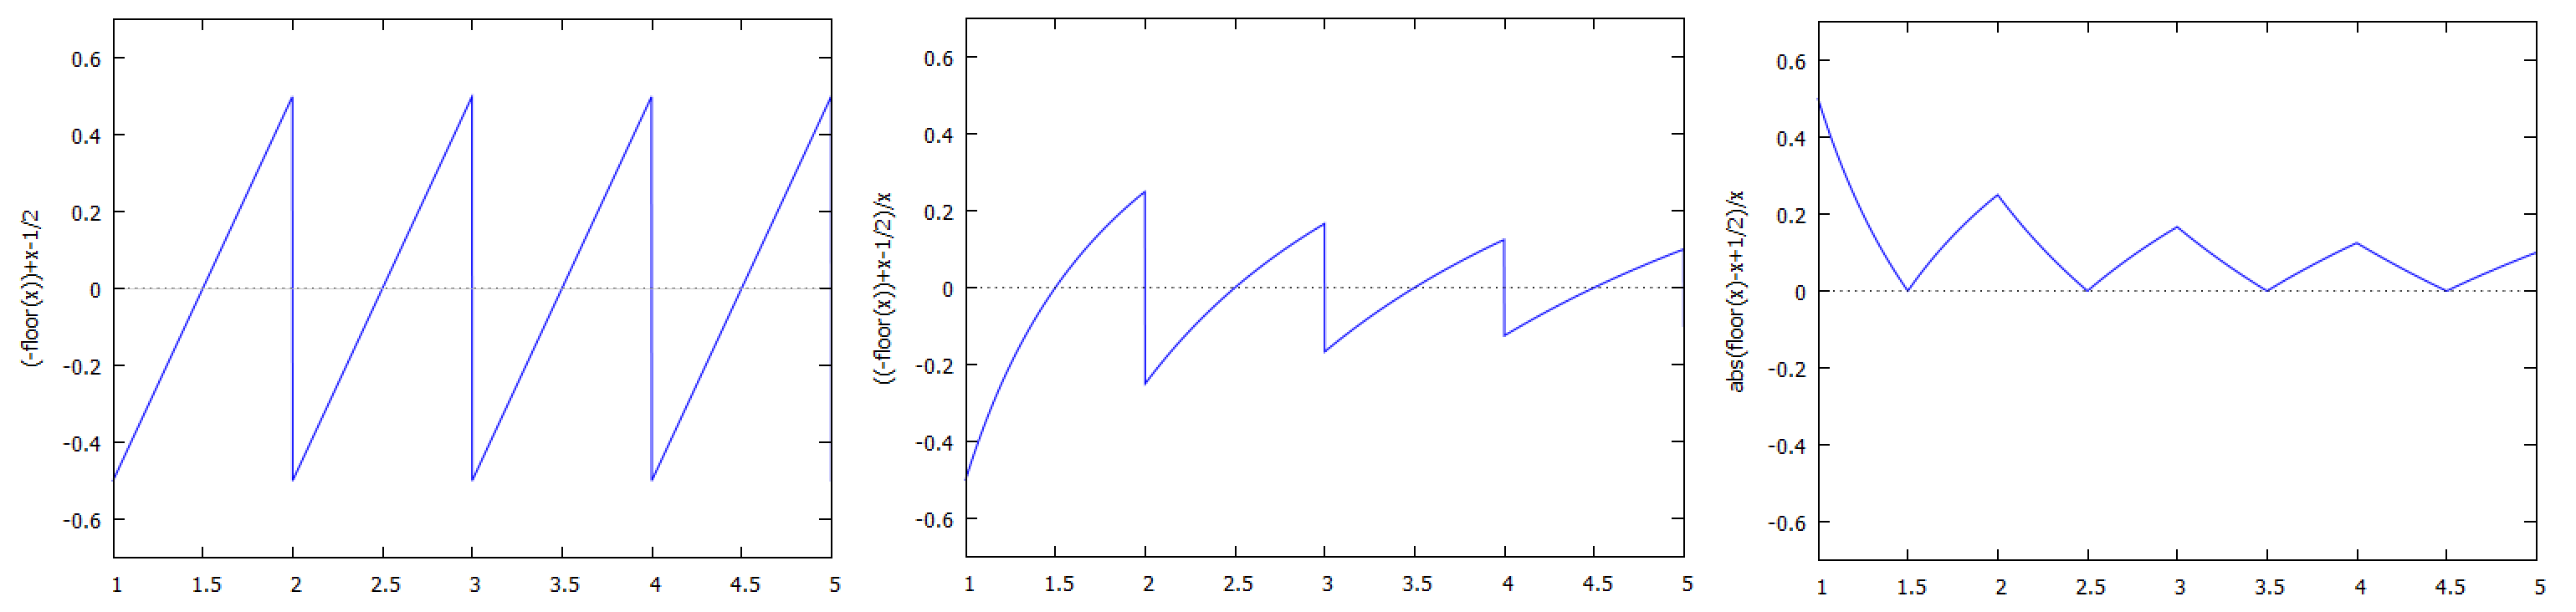
\includegraphics[width=1.00\linewidth]{B_over_x.png}
  \caption{Left is the plot of $\overline{B}_n(x) = x - [x]  -\frac{1}{2}$. Middle is $\frac{\overline{B}_n(x)}{x}$. Right is $\left|\frac{\overline{B}_n(x)}{x}\right|$}
\label{fig:B_over_x}
\end{figure}
%
{\bf Page 106}. For the first trick we have to do alternating series test to show that $\int_1^\infty$ converges. About the alternating series test, $\overline{B_1}(x)$ is the periodic function, \ie $\overline{B}_1(x) = x - [x] - \frac{1}{2}$, see Fig.~\ref{fig:B_over_x} Left. To do the alternating series test we don't actually need to do the integral. From Fig.~\ref{fig:B_over_x} Middle, we see that in each integer interval $M \le x \le M+1$, $\int_M^{M+\frac{1}{2}} \frac{\overline{B}_1(x)}{x}$ is negative and $\int_{M+\frac{1}{2}}^M \frac{\overline{B}_1(x)}{x}$ is positive. So that's your alternating series.

The alternating series test requires two conditions to be met, one the magnitude of the terms decreases and as $n\to \infty$, $a_n \to 0$. To see that $|a_n|$ decreases see Fig.~\ref{fig:B_over_x} Right, this is $ \left|\int\frac{\overline{B}_1(x)}{x}\right|$ and the second condition is obvious.

{\bf Page 108}. Mid page, in doing the integral
%
\nbea
\int_0^1 \frac{t - \frac{1}{2}}{t + s} dt
\neea
%
instead of doing IBP directly or a change of variables, it did a simple yet smart trick which actually amounts to a change of variables
%
\nbea
\int_0^1 \frac{t - \frac{1}{2}}{t + s} dt & = & \int_0^1 \frac{t +s - s - \frac{1}{2}}{t + s} dt \\
& = & \int_0^1 \frac{t + s}{t + s} dt - (s + \frac{1}{2})\int_0^1 \frac{1}{t + s} dt
\neea
%

{\bf Page 111}. In doing IBP we actually have a lot of freedom because
%
\nbea
\frac{dF(x)}{dx} = f(x) ~~~~~\longrightarrow ~~~~~ \int f(x) dx = F(x) + C
\neea
%
we have massive freedom in choosing $C$, this is true even when doing IBP. This is why the book says that ``The function $B_{2\nu} - \overline{B}_{2\nu}(x)$ is an antiderivative of $-2\nu\overline{B}_{2\nu-1}(x)$'', it is ``an'' antiderivative and not ``the'' antiderivative :) Choosing this antiderivative simplifies a lot of things, like

{\bf Page 112} Argument about the sign of $B_{2\nu} - \overline{B}_{2\nu}(x)$, this is very clever indeed, we know that the odd $\overline{B}_{2\nu+1}(x)$ has exactly three zeros at $x = 0,\frac{1}{2},1$, therefore it has two maxima and its derivative $\overline{B}'_{2\nu+1} = (2\nu + 1)\overline{B}_{2\nu}$ has 2 zeros at those maxima.

We also know that the $\overline{B}_{2\nu}$ has one maxima in $[0,1]$ because its derivative $(2\nu)\overline{B}_{2\nu - 1}$ has a zero at $x=\frac{1}{2}$, so $\overline{B}_{2\nu}$ has a maxima at $x = \frac{1}{2}$.

%
\begin{figure}
\centering
  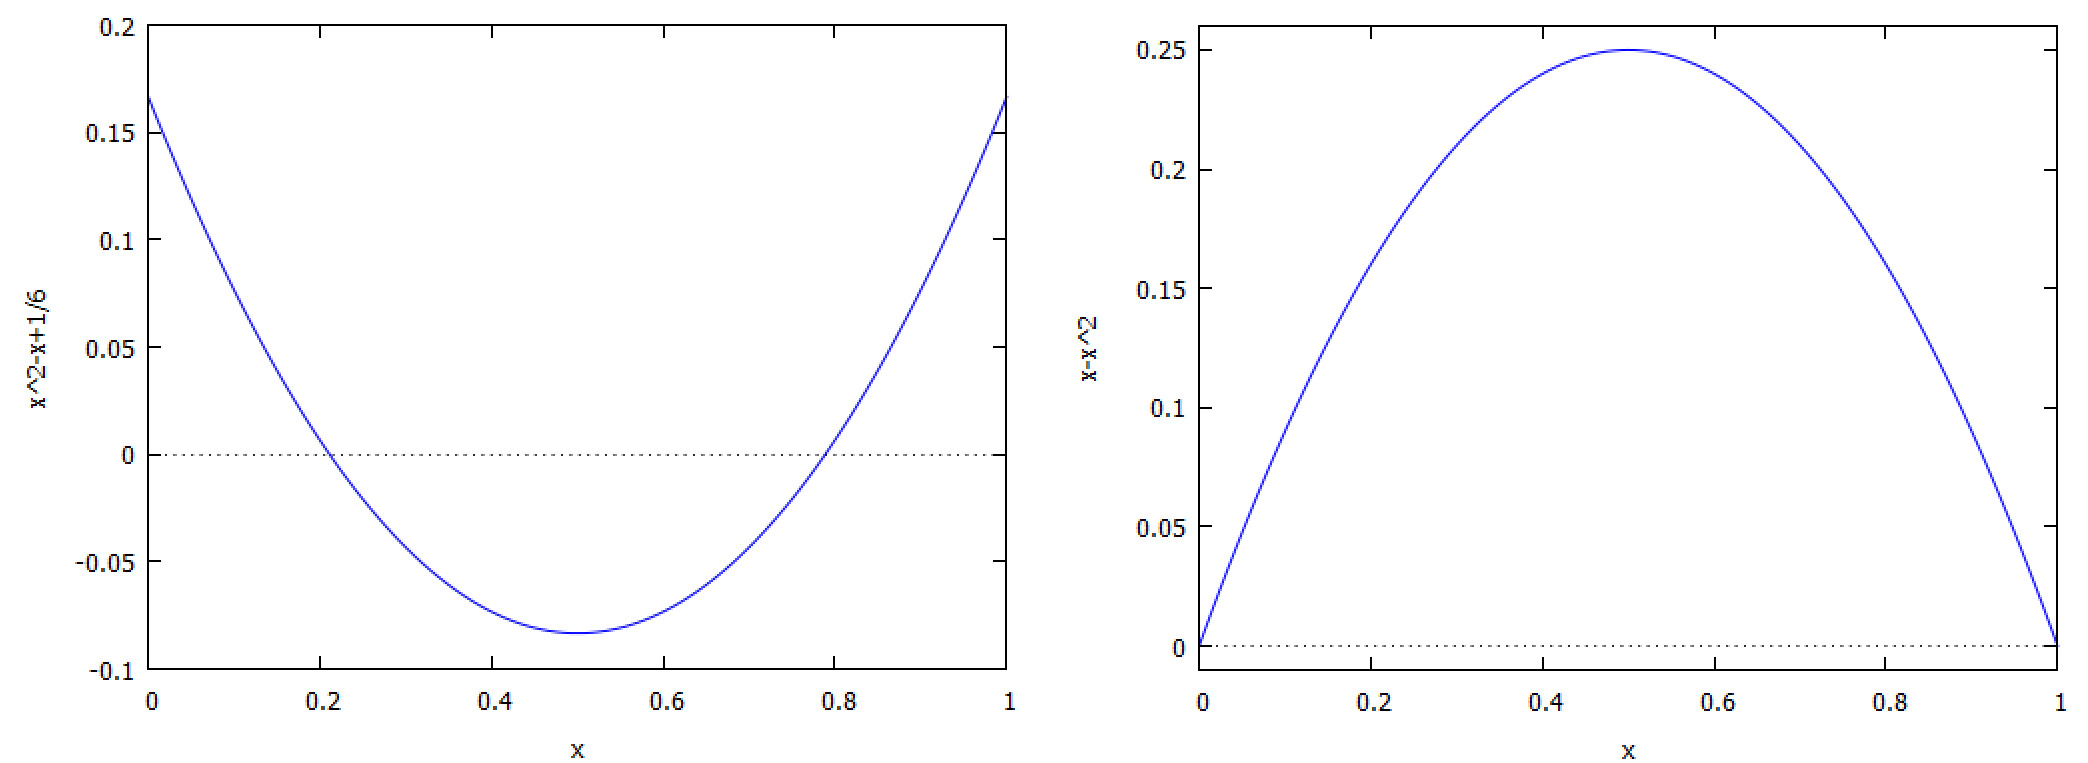
\includegraphics[width=1.00\linewidth]{B2.png}
  \caption{Left is the plot of $\overline{B}_2(x)$. Right is $B_2 - \overline{B}_2(x)$}
\label{fig:B2}
\end{figure}
%
So how do you reconcile the fact that $\overline{B}_{2\nu}$ has two zeros (not on $x=0$ or $x=1$) but only one maxima? This can be done if $\overline{B}_{2\nu}$ starts and ends off positive but in the middle it dips down to negative (or vice versa), see Fig.~\ref{fig:B2} for an example of $\overline{B}_2$. But in this case $\overline{B}_{2\nu}$ flips sign between positive and negative, we don't want this, we want the sign to stay constant throughout $[0,1]$ to simplify things. Note that we can also do $\overline{B}_{2\nu}(x) - \overline{B}_{2\nu}$ to accomplish this.


{\bf Page 113}. Last inequality
%
\nbea
\re\frac{\Pi'(\sigma + it)}{\Pi(\sigma + it)} \le 2\log t
\neea
%
In the derivation we start with the derivative of $R_0$, to do this we need to start from the very beginning at the bottom of Page 111
%
\nbea
R_{2\nu-2} & \le & \int_0^\infty \frac{[B_{2\nu} - B_{2\nu}(x)]~ dx}{2\nu (s+x)^{2\nu}}
\neea
%
we have to do the $\frac{d}{ds}$ derivative here before we take the absolute value, otherwise we incur a minus sign and we need to do the complicated $\frac{d|s|}{ds}$ later. So
%
\nbea
\frac{d}{ds} R_{2\nu-2} & \le & -\int_0^\infty \frac{[B_{2\nu} - B_{2\nu}(x)]~ dx}{(s+x)^{2\nu+1}}
\neea
%
now we can take the absolute value and get rid of the minus sign :) the next step is to estimate
%
\nbea
\frac{1}{|s+x|} \le \frac{1}{(|s|+x)\cos(\theta/2)}
\neea
%
as shown on Page 112, combining the two we get something like the middle of Page 112 (and also forgetting about the second integral)
%
\nbea
|R'_{2\nu-2}| & \le & \int_0^\infty \frac{(-1)^{\nu+1}B_{2\nu}~ dx}{\cos^{2\nu + 1}(\theta/2)(|s|+x)^{2\nu + 1}} \\
& = & \left.-\frac{|B_{2\nu}|}{(2\nu) \cos^{2\nu+1}(\theta/2)(|s|+x)^{2\nu}} \right |_0^\infty \\
& = & \frac{|B_{2\nu}|}{(2\nu) \cos^{2\nu+1}(\theta/2)|s|^{2\nu}}
\neea
%
Note that the minus sign in the second line is crucial as it negates the minus sign from computing the lower limit of the integral :) if we set $\nu=1$ we get
%
\nbea
|R'_0| & \le & \frac{B_{2}}{2 \cos^{3}(\theta/2)|s|^{2}}
\neea
%
which is what we have on Page 114. The second line on Page 114 is
%
\nbea
\left | \frac{\Pi'(s)}{\Pi(s)} - \log s \right | & \le & \frac{1}{2|s|} + \frac{B_{2}}{2 \cos^{3}(\theta/2)|s|^{2}}
\neea
%
for sufficiently large $s$ and this is the key, sufficiently large because
%
\nbea
\frac{1}{2|s|} & \ge & \frac{B_{2}}{2 \cos^{3}(\theta/2)|s|^{2}}
\neea
%
thus
%
\nbea
\left | \frac{\Pi'(s)}{\Pi(s)} - \log s \right | & \le & \frac{1}{2|s|} + \frac{1}{2|s|} \\
& \le & \frac{1}{|s|}
\neea
%
this is the second line, to get to the third line, note that
%
\nbea
\left | \frac{\Pi'(s)}{\Pi(s)} - \log s \right | & = & \left | {\re}\left(\frac{\Pi'(s)}{\Pi(s)} - \log s \right) + i \cdot \Im\left(\frac{\Pi'(s)}{\Pi(s)} - \log s \right) \right|
\neea
%
thus because we are ignoring the imaginary part
%
\nbea
\left | \re\left(\frac{\Pi'(s)}{\Pi(s)} - \log s \right) \right |  = \left | \re\frac{\Pi'(s)}{\Pi(s)} - \re\log s \right | & \le & \left | \frac{\Pi'(s)}{\Pi(s)} - \log s \right |  \\
\to \left | \re\frac{\Pi'(s)}{\Pi(s)} - \re\log s \right | & \le & \frac{1}{|s|}
\neea
%
which is the third line, also since $1 \le \sigma \le 2$, $\re\log s$ is always positive because $s$ is on the right half of the complex plane thus $\re\log s \le \log |s|$ and
%
\nbea
\re\frac{\Pi'(s)}{\Pi(s)} - \log s & \le & \left | \re\frac{\Pi'(s)}{\Pi(s)} - \re\log s \right | \\
\to \re\frac{\Pi'(s)}{\Pi(s)} - \log |s| & \le & \frac{1}{|s|} \\
\to \re\frac{\Pi'(s)}{\Pi(s)} & \le & \log |s| + \frac{1}{|s|}
\neea
%
setting $s = (\sigma + it)/2 $
%
\nbea
\re\frac{\Pi'((\sigma + it)/2)}{\Pi((\sigma + it)/2)} & \le & \log \left|\frac{\sigma + it}{2}\right| + \frac{1}{|s|} \\
& \le & \log \left|1 + i\frac{t}{2}\right| + \frac{1}{|s|}
\neea
%
now since $1 \le \sigma \le 2$ we set $\sigma = 2$, for the very last step we want to show that $\log t \ge \left|1 + i\frac{t}{2}\right|$ and $\log t \ge \frac{1}{|s|}$, the latter is obvious for sufficient large $s$, the former though
%
\nbea
\left|1 + i\frac{t}{2}\right| & = & \left (1 + \frac{t^2}{4} \right )^{1/2} \\
& = & t\left (\frac{1}{t^2} + \frac{1}{4} \right )^{1/2} \\
& \le & t
\neea
%
since whatever is in the bracket is less than 1 (again for sufficiently large $s$) and so we get the final result :)



{\bf Page 114}. Application of Euler-Maclaurin to $\zeta(s)$. This is quite straightforward except that we cannot start the sum $\sum n^{-s}$ from $n=1$ because then the series becomes
%
\nbea
\sum_{n=1}^\infty n^{-s} & = & \int_1^\infty x^{-s} dx + \frac{1}{2} 1^{-s} + \frac{B_2}{2} s + \cdots + \frac{B_{2\nu}}{(2\nu)!} s(s+1) \cdots (s+ 2\nu -2) + R_{2\nu}
\neea
%
so the series decreases only by virtue of the decrease the Bernoulli's numbers.



{\bf Page 117}. About the calculation of $n^{-\frac{1}{2} - it}$ as $n^{-1/2}[\cos(t\log n) + i\sin(t\log n)]$ as
%
\nbea
18 \log 2 & = & 4\pi -\theta \\
18 \log 3 &= & 6\pi + (\pi/3) - \theta \\
18 \log 5 & = & 9\pi + (\pi/4) - \theta
\neea
%
at first I was thoroughly confused by this but then I understood what he's trying to do, because we are calculating $\sin$ and $\cos$, we want to massage $t\log n$ in terms of special angles whose $\sin$, $\cos$ we know the value of like $\pi, \pi/3, \pi/4$, the second reason is we want to minimize $\theta$ to minimize the error. For example, $18 \log 5$ is $\sim 28.97$ so it's $9\pi + (\pi/4)$ minus some change. This is because we know $\sin$, $\cos$ of $9\pi$ and $\pi/4$. Thus
%
\nbea
\sin(9\pi + (\pi/4) - \theta) & = & \sin(9\pi + (\pi/4))\cos(\theta) + \sin(\theta)\cos(9\pi + (\pi/4)) \\
& = & -\sin(\pi/4)\cos(\theta) + \sin(\theta)\cos(\pi/4)
\neea
%
and if we minimize $\theta$ , since more than likely we calculate $\sin$, $\cos$ using the series expansion, the smaller $\theta$ is the better.

{\bf Page 119}. $\xi(s)$ is real along the vertical line $\sigma = \frac{1}{2}$, this is due to its symmetry $\xi(1-s) = \xi(s)$ and $\xi(1-s) = \Pi((1-s)/2)((1-s)-1)\pi^{-(1-s)/2}\zeta(1-s)$
%
\nbea
\xi\left(1 - \left(\frac{1}{2} + it\right)\right) & = & \Pi\left(\frac{1 - (\frac{1}{2} + it)}{2}\right)\left(1 - \left(\frac{1}{2} + it\right)-1\right)\pi^{-\left(1 - \left(\frac{1}{2} + it\right)\right)/2}\zeta\left(1 - \left(\frac{1}{2} + it\right)\right) \\
& = & \Pi\left(\frac{\frac{1}{2} - it}{2}\right)\left(\frac{1}{2} - it -1\right)\pi^{-\left(\frac{1}{2} - it\right)/2}\zeta\left(\frac{1}{2} - it\right) \\
& = & \Pi\left(\frac{\overline{\frac{1}{2} + it}}{2}\right)\left(\overline{\frac{1}{2} + it} -1\right)\pi^{-\left(\overline{\frac{1}{2} + it}\right)/2}\zeta\left(\overline{\frac{1}{2} + it}\right) \\
& = & \overline{\Pi\left(\frac{\frac{1}{2} + it}{2}\right)}  ~~\overline{\left(\frac{1}{2} + it -1\right)} ~~\overline{\pi^{-\left(\frac{1}{2} + it\right)/2}} ~~  \overline{\zeta\left(\frac{1}{2} + it\right)} \\
& = & \overline{\xi\left(\frac{1}{2} + it\right)}
\neea
%
But $\xi\left(1 - \left(\frac{1}{2} + it\right)\right) = \xi\left(\frac{1}{2} + it\right)$, therefore
%
\nbea
\xi\left(\frac{1}{2} + it\right) & = & \overline{\xi\left(\frac{1}{2} + it\right)}
\neea
%
and thus $\xi\left(\frac{1}{2} + it\right)$ is real for any real $t$. This is assuming $\zeta(\overline{s}) = \overline{\zeta(s)}$. If $\zeta(s)$ is real all along the real line then we can use the reflection principle but I'm not sure because $\zeta(s)$ has a pole at $s=1$, also for $s$ real and $s> 1$, $\zeta(s)$ is positive but for $0 < s < 1$, $\zeta(s)$ is negative, see Apostol's Theorem 13.11. For $\sigma > 1$ we know that $\zeta(\overline{s}) = \overline{\zeta(s)}$, how about for the rest $\sigma \le 1$?

Let me state the answer first and how I got it and then go for the difficulties I had. The analytically continued $\zeta(s)$ can be expanded in Laurent series about $s=1$, note that Laurent expansion is not Taylor series, it doesn't have radius on convergence since it also includes poles, so the singularities are included. To have $\zeta(\overline{s}) = \overline{\zeta(s)}$ we must have the coefficient of the Laurent series to be real
%
\nbea
\zeta(s) & = & \sum_{k=-1}^\infty a_k (s-1)^k \\
\to \overline{\zeta(s)} & = & \sum_{k=-1}^\infty \overline{a_k (s-1)^k} \\
& = & \sum_{k=-1}^\infty a_k (\overline{s}-1)^k
\neea
%
we can get to the last line only if the $a_k$'s are all real, which will be our task to show that it is so.

For $s$ real and $s > 1$, we know that $\zeta(s)$ is real, this can mean two things, either all the $a_k$'s are all real, or that the imaginary parts cancel out at the end, since $s$ is real we can split
%
\nbea
\zeta(s) & = & \Re\left\{\sum_{k=-1}^\infty a_k (s-1)^k\right\} + i\Im\left\{ \sum_{k=-1}^\infty a_k (s-1)^k \right\} \\
& = & \sum_{k=-1}^\infty a^{\rm Re}_k (s-1)^k + i\sum_{k=-1}^\infty a^{\rm Im}_k (s-1)^k \\
\to 0 & = & \sum_{k=-1}^\infty a^{\rm Im}_k (s-1)^k
\neea
%
To show that each of the $a^{\rm Im}_k$ we need a result (from algebra?) that says that a polynomial that is zero for all $x\in [c,d]$, $d > c$, must be exactly zero, \ie each coefficient is zero. While it seems intuitive I was looking for a way show it more formally somehow. The other complication here is that we start with $\frac{1}{s-1}$ instead with a constant. But an even bigger problem is that this is not just a polynomial of degree $n$, this is an infinite power series. So my meandering led me to a few things. First, let's start with the solution. What we have is an infinite power series, multiplying both sides with $(s-1)$
%
\nbea
0 & = & \sum_{k=0}^\infty a_{k-1}^{\rm Im} (s-1)^k 
\neea
%
the good news is that a Taylor series is also an infinite power series so we can think of this as a Taylor expansion of a function
%
\nbea
f(s) & = & f(1) + f'(1)(s-1) + \frac{f''(s)}{2!}(s-1)^2 + \frac{f'''(s)}{3!}(s-1)^3 + \cdots \\
& = & \sum_{k=0}^\infty a_{k-1}^{\rm Im} (s-1)^k \\
\to f^{(k)}(1) & = & a_{k-1}^{\rm Im}
\neea
%
but in the interval $s \in (1,\infty]$, $f(s) = 0$, this means $f(s)$ is a constant, which also means that its derivative is also constant, \ie 0, which means that the second derivative must be zero as well, and so on and so $f'(s) = f''(s) = \dots = f^{(k)} = 0$. Which means that each $a_{k-1}^{\rm Im} = 0$. Therefore
%
\nbea
\overline{\zeta(s)} & = & \zeta(\overline{s})
\neea
%
I initially wanted to show that this is the case through two things, one, that we know the sum $\sum_{\rho} \frac{1}{\rho}$ given in chapter 3 to be real, thus the imaginary parts have to cancel. But this doesn't mean that they come in conjugate pairs, for example  we have two complex numbers, $ae^{i\theta_a}$ and $be^{i\theta_b}$ then
%
\nbea
\frac{1}{a e^{i\theta_a}} + \frac{1}{b e^{i\theta_b}} & = & a^{-1} e^{-i\theta_a} + b^{-1} e^{-i\theta_b} \\
& = & (a^{-1} \cos(\theta_a) + b^{-1} \cos(\theta_b)) + i(a^{-1}\sin(\theta_a) + b^{-1}\sin(\theta_b))
\neea
%
and as long as $b^{-1} = -\frac{\sin(\theta_a)}{a \sin(\theta_b)}$ we have the RHS to be real but they don't form a conjugate pair.

Then I wanted to use the von-Mangoldt's $\psi(x)$ that includes $\sum_\rho \frac{x^\rho}{\rho}$, again the LHS, $\psi(x)$, is real but again, they don't need to form conjugate pairs to cancel out, they just need to cancel out like above, just messier algebra
%
\nbea
\frac{x^{\sigma_1 + it_1}}{\sigma_1 + it_1} + \frac{x^{\sigma_2 + it_2}}{\sigma_2 + it_2} & = & \frac{x^{\sigma_1 + it_1}}{\sigma_1^2 + t_1^2} + \frac{x^{\sigma_2 + it_2}}{\sigma_2^2 + t_2^2} = \frac{x^{\sigma_1 + it_1}}{\rho_1^2} + \frac{x^{\sigma_2 + it_2}}{\rho_2^2} \\
& = & \frac{\rho_2^2 x^{\sigma_1} \cos(t_1 \log x) + \rho_1^2 x^{\sigma_2} \cos(t_2 \log x) + i (\rho_2^2 x^{\sigma_1} \sin(t_1 \log x) + \rho_2^2 x^{\sigma_2} \sin(t_2 \log x))}{\rho_1^2\rho_2^2}
\neea
%
by adjusting $t_1$ or $t_2$ we can cancel the imaginary part but they don't have to be a conjugate pair.

\bigskip
\underline{\textbf{\textit{Erroneous Excursions}}}

So I initially wanted to show the above by showing that if a polynomial of degree $N$ is zero in the interval $[c,d]$ then it must be exactly zero, although the proof below should be OK, it doesn't apply to an infinite power series, which can also be seen from how the proof goes.

{\bf Polynomial Proposition}. Suppose that a polynomial of degree $N$, $\sum_{n=0}^N b_n y^n$ is zero for all $y \in [c,d]$. We can think of the polynomial as a function $f(y) = \sum_{n=0}^N b_n y^n$ then for this interval the function $f(y)$ is constant (which is zero in this case). This also means that the derivative $f^{(1)}(y)$ 
%
\nbea
f^{(1)}(y) & = & \sum_{n=1}^N n b_n y^{n-1} = 0
\neea
%
is also zero in this interval (sans the endpoints). Repeating the argument $N-1$ times we get $f^{(N-1)}(y) = N! b_N = 0$, which means that the highest coefficient $b_N$ is zero. Going back to the beginning, repeating the arguments over again we get $b_{N-1} = 0$, $b_{N-2} = 0, \dots b_0 = 0$, \ie each of the coefficient to be zero, thus the whole polynomial is exactly zero.

We can apply the same argument for a polynomial that is equal to a constant instead of zero, $\sum_{n=0}^N b_n y^n = C$. We just need to set $b_0 \to b_0 - C$, again, each coefficient must be zero, including $b_0 - C = 0$, thus the polynomial is just a constant $b_0 = C$.

We can employ the same strategy for a polynomial that starts with a negative power $\sum_{k=-M}^N b_k y^k$, since the whole thing is equal zero we just need to multiply the whole thing with $y^M$, if the interval contains zero we just need to split the interval $[c,0),(0,d]$ to avoid multiplying by zero and focus on one of them since if it is exactly zero in one of the intervals, then it is zero everywhere.

{\bf Another Fundamental Proposition}. We can use the above differentiation strategy to show a weaker form of the fundamental theorem of algebra, \ie a polynomial of degree $n$ has at most $n$ real roots. The fundamental theorem asserts there are exactly $n$ complex roots but we are only interested in reality :)

We can use the above together with induction and an observation that to have more than one zeros we must have extremum points.

Induction base is the case of polynomial of degree one, $a_1 x + a_0 = 0$, thus there is only one zero at $x = -a_0/a_1$. Inductive hypothesis is that up to degree $N$ the number of roots is at most the degree of the polynomial. Now we tackle $N+1$. Between any two consecutive zeros there must be an extremum between them, \ie the derivative must have a zero between them. But the derivative of a polynomial of degree $N+1$ is a polynomial of degree $N$ and by the inductive hypothesis this polynomial can have at most $N$ zeros, since the number of zeros is just the number of extrema plus one, the original polynomial of degree $N+1$ can at most have $N+1$ zeros. The argument still applies in even the case where we have multiple roots, in this case the roots are at the extremum itself.

As to why they always have roots complex roots, intuitively you can see that since a polynomial is analytic, it obeys the Riemann-Cauchy condition, \ie it's a harmonic function, therefore a maxima in the real line must be a minima in the imaginary line, since a holomorphic function cannot have true maxima/minima, it only has saddle points thanks to Riemann-Cauchy equation.

Other ways I was trying to show that $a_{k}^{\rm Im} = 0$, is to calculate the analytically continued integral explicitly as a function of $s$. There are at least a couple of difficulty with this
%
\begin{enumerate}
%
\item We need to set the value of $s$ before doing the integral $\int_{+\infty}^{+\infty}\frac{(-x)^{s-1}}{e^x - 1}$. We can't just integrate it and then set $s$, this is especially true for the small circle integral as we will see.
%
\item Even if we can do the integral first, doing the integral itself doesn't really give anything useful, one problem is that the final result must be independent of the small circle radius $c$, but to show that this is so is not straightforward.
%
\end{enumerate}
%
Let's see what happens when we integrate the small circle, we can actually do this with the help of the Bernoulli numbers
%
\nbea
\lim_{\epsilon\to0} \int_{0+\epsilon}^{2\pi-\epsilon} \frac{(-x)^{s}}{e^x - 1} \frac{dx}{x} & = & \lim_{\epsilon\to0} \int_{0+\epsilon}^{2\pi-\epsilon} (-x)^{s-2}\frac{x}{e^x - 1} dx \\
& = & \lim_{\epsilon\to0} \int_{0+\epsilon}^{2\pi-\epsilon} (-x)^{s-2} \sum_{n=0} \frac{B_n x^n}{n!} dx \\
& = & \lim_{\epsilon\to0} \sum_{n=0} (-1)^{s}\int_{0+\epsilon}^{2\pi-\epsilon} \frac{B_n x^{s+n-2}}{n!} dx \\
& = & \lim_{\epsilon\to0} \sum_{n=0} (-1)^{s} i \int_{0+\epsilon}^{2\pi-\epsilon} \frac{B_n (ce^{i\theta})^{s+n-2}}{n!} (ce^{i\theta}) d\theta \\
& = & \lim_{\epsilon\to0} \sum_{n=0} (-1)^{s} \frac{B_n c^{s + n - 1}}{n! (s + n-1)} (e^{i (2\pi - \epsilon)(s+n-1)} - e^{i (0 + \epsilon)(s+n-1)}) \\
& = & \sum_{n=0} (-1)^{s} \frac{B_n c^{s + n - 1}}{n! (s + n-1)} (e^{i 2\pi (s+n-1)} - 1)
\neea
%
Here we see the first problem, if we set $s$ to be a negative integer before the integration we will get the values of $\zeta(-n)$ but if we do it after the integration we will just get zero since $e^{2\pi i(s + n - 1)} = 1$ if $s + n - 1$ is an integer.

Say $s$ is not an integer so we can still do the integral, the problem is that this is a function of $c$ (and it is obvious that the complex conjugate of this integral is not the same as the integral of $\overline{s}$ because conjugating $e^{2\pi i(s + n - 1)}$ will not only turn $s \to \overline{s}$ but also adding a negative sign in front of the $i$).

To remove the dependency on $c$, we can integrate the rest of the integrals $\int_c^\infty \frac{(-x)^{s-1}}{e^x - 1}$, however, if we expand it using Bernoulli's numbers, the final integral we get will be of the form $\int_c^\infty x^{s + n -2}$ and the upper limit will give us issues.

{\bf Page 119, Footnote}. $Z(t)$ is real when $t$ is real, we can see this easily from 
%
\nbea
\xi\left(\frac{1}{2} + it\right) & = & \left \lbrack e^{\re \log \Pi(s/2)} \pi^{-1/4} \frac{-t^2 - \frac{1}{4}}{2} \right \rbrack Z(t)
\neea
%
since the LHS is real and the first term on the RHS is real, $Z(t)$ must be real as well.

{\bf Page 120}. The goal here is to express everything in terms of powers of $\left(\frac{1}{t}\right)$.










About the symmetry of $\frac{\xi'(s)}{\xi(s)}$, for simplicity let's denote $\frac{\xi'(s)}{\xi(s)} = F(s)$,
%
\nbea
\int_{1\tfrac{1}{2}}^{1\tfrac{1}{2} + iT} F(s) ds & = & i \int_{0}^{T} F(1\tfrac{1}{2} + it) dt
\neea
%
while on the opposite side we have
%
\nbea
\int_{-\frac{1}{2} + iT}^{-\frac{1}{2}} F(s) ds & = & i \int_{T}^{0} F(-\tfrac{1}{2} + it) dt
\neea
%
next is to use the symmetry $\xi(s) = \xi(1-s)$ but we need to be careful in using the symmetry for $F(s)$ becaue for the derivative $\xi'(s)$
%
\nbea
\left. \frac{d}{ds} \xi(s) \right|_{s = w} & = & -\left. \frac{d}{ds} \xi(s) \right|_{s = 1 - w}
\neea
%
this is analogous to our familiar friend the cosine function, even though it's symmetric with respect to the $y$ axis it's derivative is the opposite of one another across the vertical axis
%
\nbea
\left. \frac{d}{dx}\cos(x) \right|_{x = y} & = & -\left. \frac{d}{dx}\cos(x) \right|_{x = -y}
\neea
%
Therefore, since $\xi(s) = \xi(1-s)$ we have $\frac{\xi'(1-s)}{\xi(1-s)} = F(1-s) = -F(s)$ so the second integral becomes
%
\nbea
i \int_{T}^{0} -F(1 - (-\tfrac{1}{2} + it)) dt & = & i \int_{0}^{T} F(1\tfrac{1}{2} - it) dt = i \int_{0}^{T} F(\overline{1\tfrac{1}{2} + it}) dt \\
& = & i \int_{0}^{T} \overline{F(1\tfrac{1}{2} + it)} dt \\
& = & i \left  ( ~\overline{\int_{0}^{T} F(1\tfrac{1}{2} + it) dt } ~ \right )
\neea
%
Now, what we originally want was $\Im[\int_C F(s)]$, since there is a factor of $i$ in front of the integral what we really want is the real part, but
%
\nbea
\re\left  ( ~\overline{\int_{0}^{T} F(1\tfrac{1}{2} + it) dt } ~ \right ) & = & \re \left  ( ~\int_{0}^{T} F(1\tfrac{1}{2} + it) dt ~ \right )
\neea
%
and so the two integral along the vertical segments are equal.

We now need to show that the integral on the two horizontal segments are equal, the steps are similar, on the right segment we have
%
\nbea
\int_{1\tfrac{1}{2}}^{\tfrac{1}{2}} F(x + iT) dx
\neea
%
while on the left segment we have
%
\nbea
\int_{\tfrac{1}{2}}^{-\tfrac{1}{2}} F(x + iT) dx
\neea
%
using $F(1 - s) = -F(s)$
%
\nbea
\int_{\tfrac{1}{2}}^{-\tfrac{1}{2}} F(x + iT) dx & = & \int_{\tfrac{1}{2}}^{-\tfrac{1}{2}} -F(1-x - iT) dx, ~~~~~ y = 1-x \\
& = & \int_{\tfrac{1}{2}}^{1\tfrac{1}{2}} F(y - iT) dy = \int_{\tfrac{1}{2}}^{1\tfrac{1}{2}} F(\overline{y + iT}) dy \\
& = & -\left ( ~ \overline{\int_{1\tfrac{1}{2}}^{\tfrac{1}{2}} F(y + iT) dy} ~ \right ) \\
\neea
%
in this case since there's no $i$ multiplying it we want the imaginary part of the integral and the overall minus sign helps us because the complex conjugate adds an extra minus sign to the imaginary part thus
%
\nbea
\Im\left \lbrack - \left ( ~ \overline{\int_{1\tfrac{1}{2}}^{\tfrac{1}{2}} F(y + iT) dy} ~ \right ) \right \rbrack & = & \Im \left \lbrack \int_{1\tfrac{1}{2}}^{\tfrac{1}{2}} F(y + iT) dy \right \rbrack
\neea
%
and the integrals along the two segments are equal.

\bigskip
\underline{\textit{\textbf{Branches and Cuts}}}. I initially wanted to show the above symmetry using the Fundamental Theorem of Calculus. Since the integrand is nothing but $\frac{d\log\xi(s)}{ds}$, if we integrate it we just get back $\log\xi(s)$. But this is a dangerous thing to do since $\log\xi(s)$ has many branch points, one for each of the zeros of $\xi(s)$.

A pertinent example would be $\log\left ( \tfrac{z+1}{z-1}\right )$


\bigskip
\underline{\textit{\textbf{Brief (Pedestrian) Review of Branches and Cuts}}}. We have branches because we have multi-valued functions. If we restrict the function to be single valued, it is said that we are choosing a branch. For example, how do we create single-valued functions out of $f(z) = z^{1/3}$?

One way is by creating three different single-valued functions, $f_1(z) = |z|^{1/3}e^{i\bar\theta/3}$, $f_2(z) = |z|^{1/3} e^{i\bar\theta/3 + 2\pi i/3}$ and $f_3(z) = |z| e^{i\bar\theta/3 + 4\pi i / 3}$ where $z = |z| e^{i\theta}$ and $\bar\theta = \theta \pmod{2\pi}$. 

The first, $f_1(z)$ will generate numbers with angle $0 \le \arg (f_1(z)) < \tfrac{2\pi}{3}$, the second $f_2(z)$ generates $\tfrac{2\pi}{3} \le \arg (f_2(z)) < \tfrac{4\pi}{3}$ and the third $f_3(z)$ produces numbers with $\tfrac{4\pi}{3} \le \arg (f_3(z)) < \tfrac{6\pi}{3}$. This way we cover all possible values of $z^{1/3}$.

Rather than splitting the function into three single valued ones we can split the domain into three complex planes. Let's take a simpler example of $z^{1/2}$. We can again create two single valued functions $f_R(z) = |z|^{1/2} e^{i\bar\theta/2 -\pi i/2}$ whose output is in the right half plane and $f_L(z) = |z|^{1/2} e^{i\bar\theta/2 + \pi i/2}$ whose output is in the left half plane.

But wouldn't it be simpler if we can just designate $f(z) \to |z|^{1/2} e^{i\theta/2}$ while still maintaining the output to be always say for instance on the right half of the plane? This looks a lot more natural since taking a square root is (primarily) just multiplying the exponent by $\tfrac{1}{2}$.

We can do this by setting the domain to be $z = |z|e^{i\theta}$ where $\theta$ is now restricted to $\theta \in (-\pi,\pi)$, since the interval is open, this is equivalent to excluding the negative real axis. With this choice of domain our $f_R$ simply becomes $f_R(z) = |z|^{1/2} e^{i\theta/2}$ which is very natural (compared to $f_R(z) = |z|^{1/2} e^{i\bar\theta/2 -\pi i/2}$).

What we are doing is essentially creating two copies of the complex plane, one for $f_R$ and another for $f_L$, In their own planes, $f_R$ and $f_L$ take the same form $f_L(z) = f_R(z) = |z|^{1/2} e^{i\theta/2}$. However, the argument of $z$ is now different in these two planes.

In the $f_R$ plane, $\theta \in (-\pi, \pi)$ and in the $f_L$ plane $\theta \in (-3\pi, -\pi)$ (we are excluding the negative real axis). These choices of angles make sense, by limiting $\theta \in (-\pi, \pi)$ we essentially limit $ -\frac{\pi}{2} < \arg(f_R(z)) < \frac{\pi}{2}$, which is the right half of the plane, and $\theta \in (-3\pi, -\pi)$ means $ -\frac{\pi}{2} < \arg(f_L(z)) < -\frac{3\pi}{2}$ which is the left half of the plane.

To make things clearer, in the $f_R$ plane we start the angle from slightly above the negative real axis with $\pi$, we then go clockwise, the positive real axis has the angle zero and when we reach slightly below the negative real axis we get $-\pi$. For the $f_L$ plane we start slightly above the negative real axis with $-\pi$ going clockwise, the positive real axis is now at angle $-2\pi$ and when we are at slightly below the negative real axis we are at $-3\pi$.

Now, just because $\theta \in (-3\pi, -\pi)$ in the $f_L$ plane, it doesn't mean that $w_L = f_L(z)$ cannot have $\arg(w_L)$ bigger than $-\pi$, for example, $f_L(e^{-i\pi}) = e^{-i\pi/2}$, this is fine since this is the angle of $w_L$ and not of $z$, we only restrict the angle of $z$.

From the illustration above it is clear that if we start with the $f_R$ plane at slightly above the negative real axis and go clockwise one round and still continues to more negative angles $< -\pi$ we are crossing into the $f_L$ plane. The negative real axis that we exclude is called a branch cut. Intuitively it is where we glue together the two planes as illustrated above. So if we cross it, our single valued function will evolve into another (different) one, this is why we are not supposed to cross the branch cut whether when we're doing integral or not.

For our first example $z^{1/3}$, instead of defining three separate single-valued functions like before, we can create three separate planes which can be affected by restricting the angle of $z$.

Recall that $f_1(z) = |z|^{1/3}e^{i\bar\theta/3}$, \ie the output of this function has angle $0 \le \arg(f_1(z)) < \frac{2\pi}{3}$ a.k.a the first $120^\circ$ pizza slice and the other two $f_2$ and $f_3$ has output in the subsequent $120^\circ$ pizza slices respectively. We can instead have $f_{1,2,3}$ all have the same form $|z|^{1/3} e^{i\theta/3}$ by defining a branch cut $\theta \in (0, 2\pi)$ which excludes the positive real axis.

Let's verify the outcome, well, $f_1$ is obvious, $f_2$ we get by going to the second plane which is $\theta \in (2\pi, 4\pi)$ so that $\frac{2\pi}{3} < \arg(f_2) < \frac{4\pi}{3}$ which is the second $120^\circ$ pizza slice and to get $f_3$, again, we cross the branch cut a second time from $f_2$ plane going to $f_3$ plane, this time we restrict $\theta \in (4\pi, 6\pi)$ so that $\frac{4\pi}{3} < \arg(f_2) < \frac{6\pi}{3}$ which is the last $120^\circ$ pizza slice. If we cross the branch cut again, we will end up in $f_1$'s plane but this time we have $\theta \in (6\pi, 8\pi)$ with the resulting output $\frac{6\pi}{3} < \arg(f_1) < \frac{8\pi}{3}$ which is the first pizza slice again :)

So that's the story on how we got branch cuts and how it relates to multi-valued functions. In essence
%
\begin{enumerate}
%
\item If we have a multi-valued function, we need to make it single-valued.
%
\item We can either explicitly generate different single-valued functions or restrict the domain using branch cuts.
%
\item Branch cuts are the way to go, this way we create multiple complex planes, one for each of the single valued functions, and in this way all of the single-valued functions have the same form.
%
\item We must not cross branch cuts because then we are going into a different plane and therefore a different function (although the function has the same form).
%
\item Branch cuts need not be straight lines and they don't have to be on the real axis, they can be some wavy lines as long as they end on a branch point and not cross each other.
%
\item The final goal is to make the function single-valued and analytic, so it's not about assigning angles to $z$, we do it to make the function well-behaved, we'll see an example later.
\end{enumerate}
%

Talking about branch points, in the above examples of $z^{1/2}$ and $z^{1/3}$, the branch points are $z = 0$ and $z = \infty$. What is a branch point? A branch point can be defined (at least) two ways. The first not so pedestrian definition is that it is a point $z_0$ where for any $\epsilon > 0$, $f(z)$ is multivalued for all points in its neighborhood, \ie all $z$ such that $|z - z_0| \le \epsilon$.

The more pedestrian definition is, a branch point is a point where the multi-valued function stopped being multi-valued. An even more pedestrian definition is that a branch point is a point we use to define other points, this is what we usually do to calculate things. Let's see how this goes.

The above way of restricting the angle, $\theta \in (0,2\pi)$ for example, is not the best way of expressing how to calculate with a branch cut. A better way is to first pick a branch point and then use it as a reference to define other points in the domain. Let's take $(z-1)^{1/2}$ for example.

The branch point here is $z=1$ because here the function stops being multi-valued. We can then express all other points with respect to $z = 1$. Note that numbers in the complex plane are like vectors, so if we choose $z=1$ as a reference, all other points can be expressed as $z = 1 + r e^{i\alpha}$ where $r = |z - 1|$ and $\alpha$ is the angle we need to define to make things work.

To define this angle $\alpha$, we first need to choose a branch cut. Say we choose the cut to be the real axis with $\re(z) > 1$, it doesn't mean that the angle has to be $(0,2\pi)$. We can still assign $(-\pi,\pi)$ even though this means that the angle sort of cuts through the cut, this is fine.

The problem with $(-\pi, \pi)$ is that at $z = 0$, $(z-1)^{1/2}$ will have a discontinuity, because at $z = 0^+$ we get $(0^+-1)^{1/2} = 1 + e^{i\pi/2}$ while at $z = 0^-$ we have $(0^--1)^{1/2} = 1 + e^{-i\pi/2}$. This was my big misunderstanding that I thought the angle assignments must not cut across the cut, rather it must make the function well behaved.

To see an example of angle assignment that cuts through the branch cut but still makes the function well behaved we go to the next non-trivial example, $\log \left ( \frac{z+1}{z-1}\right )$.

This time we have two branch points, $z = 1$ and $z = -1$. The most common choices of branch cuts are a cut from $-1$ to $+1$ or a cut from $-1$ to $-\infty$ and $+1$ to $+\infty$. We'll go through both of them.

For the first choice, we define the angles like shown, to make

 


As an application of what we learned above let's see what happens when we have a multi-valued function inside an integral and as a result of an integral. We'll start with a simple example and move on to more complicated ones.





Analytic continuation, we can continue $\log_{(-\pi,\pi)}$ with $\log_{(0,2\pi)}$ because they have the same value in the upper half plane.






The way we do branch cuts



Example of multi-valued function in an integral and as a result of an integral (Fundamental Theorem).

It's not always straightforward as to what to do to split the angle, especially when we have many branch points, a pertinent example would be $\log\left ( \tfrac{z+1}{z-1}\right )$













$z^p$ has branch points at 0 and infinity, at infinity because $z^p = e^{p \log z}$ and log $z$ has branch points at 0 and infinity through $\log \tfrac{1}{z} = -\log z$



The branches dictate the angle assignment, not the other way round

Each branch is on its own sheet and single valued. Connected through the cut, this is why we cannot go across the cut since then we are going to a different branch of the function which is a different function. Give example.

Can only use fundamental if the function is fundamental, thus must choose a branch and a cut.

The expansion of $(z^2 - 1)^{\tfrac{1}{2}}$ is $z - \frac{1}{2z} + \dots$










So you don't want $\zeta$ to be 0 along $C$ but you only want $\re \zeta(s)$ to be zero. But beyond $\re(s) > 1$ there's no zero.




Baclund's estimate of $N(T)$, towards the end it has
%
\nbea
\left | \re\zeta(2 + iT)\right | & \ge & 1 - \frac{1}{2^2} - \frac{1}{3^2}- \frac{1}{4^2} - \dots
\neea
%
This is because
%
\nbea
\re\zeta(2 + iT) & = & \sum_{n=1}^\infty n^{-2} \cos(T\log n) \\
& = & 1 + \sum_{n=2}^\infty n^{-2} \cos(T\log n) \\
& \ge & 1 + \sum_{n=2}^\infty n^{-2} (-1)
\neea
%
as $cos \ge -1$.



































%
\begin{figure}
\centering
  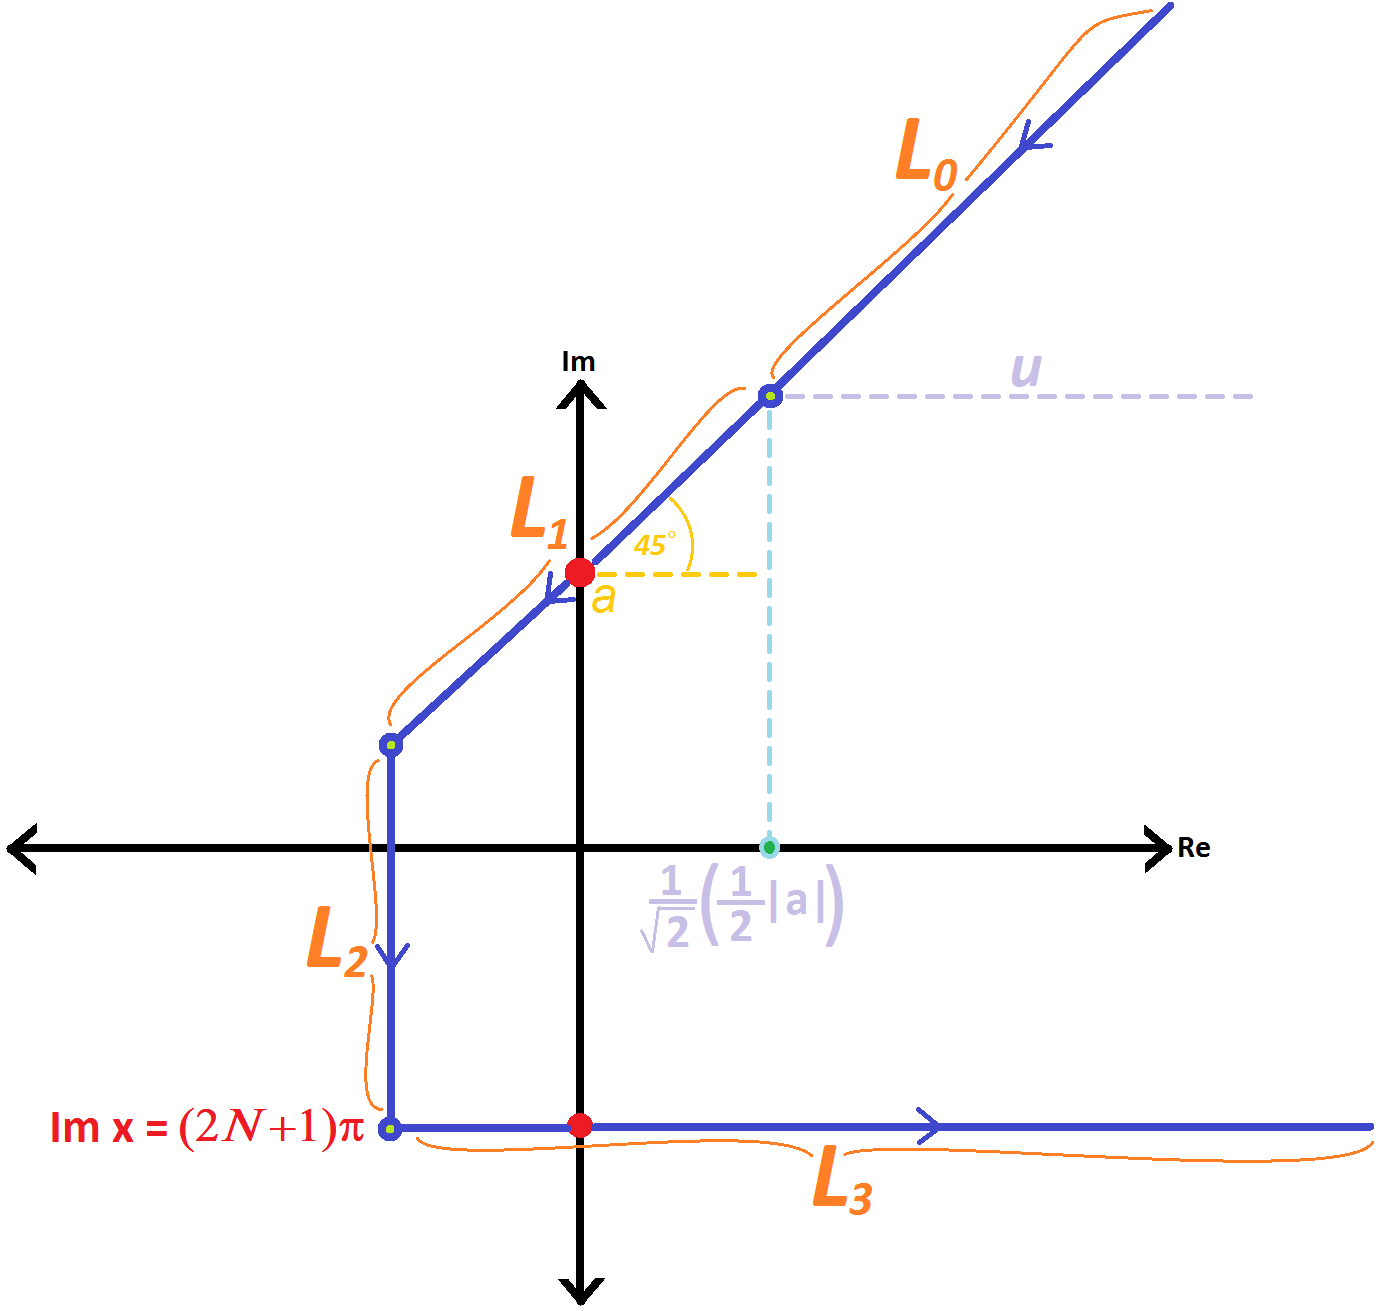
\includegraphics[width=1.00\linewidth]{Saddle_Point_Contour.png}
  \caption{Contour of integration used for the saddle point method.}
\label{fig:Saddle_Point_Contour}
\end{figure}
%





{\bf Page }. We don't have to use Taylor expansion, we just need to massage it into a power series.













{\bf Page }. So the contour used for this saddle point is a peculiar one, see Fig.~\ref{fig:Saddle_Point_Contour}, it starts from infinity, $a + \infty\cdot e^{i\pi/4}$ to $a - \frac{1}{2}|a|e^{i\pi/4}$, vertically down to the line $Im(x) = (2N+1)\pi$ and to infinity again on this same line. The goal is to show that only the integral on the segment $L_1$ is significant.

To make sense of this integral, first do the following variable substitution, $x = a + k e^{i\pi/4}, dx = dk$ with $a = i(2\pi t)^{1/2}$ and $k$ starting from $\frac{1}{2} |a|$, again see Fig.~\ref{fig:Saddle_Point_Contour}, note also that we are taking the modulus, so we can flip the integration direction to go from $a$ to infinity rather than from infinity to $a$, therefore the integral becomes
%
\nbea
\left | \int_{L_0} \frac{dx}{e^x - 1} \right | = \left | \int_{-L_0} \frac{dx}{e^x - 1} \right | & \le & \int_{L_0} \frac{|dx|}{|e^x - 1|} \\
& = & \int_{\frac{1}{2}(2\pi t)^{1/2}}^\infty \frac{|dk|}{|e^x - 1|} \\
& = & \int_{\frac{1}{\sqrt{2}}(\pi t)^{1/2}}^\infty \frac{dk}{|e^{a + k e^{i\pi/4}} - 1|}
\neea
%
Now we use the less famous triangle inequality $|a- b| \ge |a| - |b|$
%
\nbea
|e^{a + k e^{i\pi/4}} - 1| & \ge & |e^{a + k e^{i\pi/4}}| - 1 \\
& = & |e^{a}||e^{k \cos (\pi/4) + i k \sin(\pi 4)}| - 1 \\
& = & e^{\frac{1}{\sqrt{2}}k } - 1
\neea
%
We can now do another variable change $u = \frac{1}{\sqrt{2}} k, dk = \sqrt{2} du$ and the integral becomes
%
\nbea
\int_{\frac{1}{\sqrt{2}}(\pi t)^{1/2}}^\infty \frac{dk}{e^{\frac{1}{\sqrt{2}}k } - 1} & = & \int_{\frac{1}{\sqrt{2}}\frac{1}{\sqrt{2}}(\pi t)^{1/2}}^\infty \frac{\sqrt{2} du}{e^{u} - 1} \\
& = & \int_{\frac{1}{2}(\pi t)^{1/2}}^\infty \frac{\sqrt{2} du}{e^{u} - 1} \\
& = & \int_{\frac{1}{2}(\pi t)^{1/2}}^\infty \frac{e^{-u}\sqrt{2} du}{1 - e^{-u}}
\neea
%
The way I figured out this integral is by noting that integration along $k$ is somewhat like integration along the dotted line $u$ in Fig.~\ref{fig:Saddle_Point_Contour} but we need to of course take care of the fact that (from the triangle they form) the line $u$ is $\frac{1}{\sqrt{2}} k$.










{\bf Page }. Dealing with log in the complex plane is a bit tricky, we usually have to designate a cut to avoid certain numbers having multiple log values, for example, 1 can be represented by $e^{i0}$ or $e^{i2\pi}$, the log of which are $0$ and $i 2\pi$ respectively. If we made the cut along the positive real axis we prevent $e^{i0}$ to becoming $e^{i2\pi}$, if the cut is on the negative real axis we prevent $e^{i\pi}$ from becoming $e^{-i\pi}$ while the positive real axis is set to be $r e^{i0}$, we can set other conventions of course even with the same cut.

But in this case we are not bothered by this, I initially wrongly thought that the reason the starting point of $L_2$ cannot have the min $\Im(\log(-x))$ was because in this case $-x$ would be in the south east quadrant and the integration contour $C_M$ dictates that we make the cut on the positive real axis, so we have $0 \le \theta < 2\pi$ starting from the positive real axis going counter clockwise. In this south east quadrant the argument of $-x$ would be near $2\pi$. While the end point of $L_2$ would have $-x$ in the north east quadrant, thus the argument of $-x$ would be the smallest.

Then I thought maybe the starting point of $L_2$ has the smallest argument because
%
\nbea
\Im{(\log(-x))} & = & \Im{(i\pi + \log(x))}
\neea
%
so to minimize $\Im(\log(-x))$ is the same as minimizing the argument of $x$ and since the starting point of $L_2$ is in the north west quadrant it has the smallest argument, again assuming the cut is in the positive real axis.

But I was wrong, this is just about a lower bound, we don't care about cut here. If you see the derivation he just wanted the most negative argument of all, since the starting point of $L_2$ has $-x$ in the south east quadrant, its argument is negative while its end point in the north east quadrant would have a positive argument so we chose the one with the negative argument, that's all.










Lesson of the day, doing integrals without doing integrals.


We Taylored $\Psi(p+y)$ around $p$
%
\nbea
\Psi(p+y) & = & \Psi^{(0)}(p) + \Psi^{(1)}(p) (y+p - p) + \frac{1}{2!}\Psi^{(2)}(p) (y+p - p)^2 + \dots \\
& = & \sum_{k=0}^\infty \frac{\Psi^{(k)}(p)}{k!} y^k
\neea
%




`` $\dots$ and in which sum is finite'', ``which'' here refers to $\sum_{j=0}^\infty A_j \omega^j$


So the goal here is to calculate $b_0 c_0 + b_1 c_1 + \dots + b_Kc_K$, but the way Riemann did it is not to calculate this sum at all, the way he did it was to calculate an approximation to this sum by expressing it in terms of a power series of $\omega^j$. I say an approximation because $b_K$ contains $\omega_K$ while we are only mucking around with $\omega^\nu$ where $K$ is large enough such that $b_{K+1}, b_{K+2}, \dots$ does not contain $\omega^\nu$.

This is what confused me when he expressed $G(y)$ as $\sum_{j=0}^\infty A_j \omega^j$ and he was only concerned about $A_0, A_1, \dots, A_{\nu-1}$ that are not dependent on $K$. Why care only up to $A_{\nu-1}$, the goal here is to calculate $b_0 c_0 + b_1 c_1 + \dots + b_Kc_K$, we need the $A$'s so that we can get the coefficient of negative powers of $y$ so that we can combine them with positive powers of $y$ in $\sum_{k=0}^\infty \frac{\Psi^{(k)}(p)}{k!} y^k$ to get the coefficient of $y^0$, but the coefficient of $y^0$ is exactly $b_0 c_0 + b_1 c_1 + \dots + b_Kc_K$, it includes $\omega^K$, so I figured that what we are doing here is an approximation of $b_0 c_0 + b_1 c_1 + \dots + b_Kc_K$.



%
\nbea
(2y)^{n-1}(n+1)b_{n+1}
\neea
%















res f, only is f is holomorphic, no branch cut nothing























\end{document}